%% Copyright (C) 2018 Adrien Blanchet 
%% 

%%%%%%%%%%%%%%%%%%%%%%%%%%%%%%%%%%%%%%%% 
% Chapitre 2 % 
%%%%%%%%%%%%%%%%%%%%%%%%%%%%%%%%%%%%%%%% 

\chapter{L'expérience Stereo} 
\label{chap:chapitre_2} 

\citationChap{ 
Oser ; le progrès est à ce prix. Toutes les conquêtes sublimes sont plus ou moins des prix de hardiesse. 
}{Victor Hugo}{Les Misérables III : Marius} 

\minitoc 

\newpage 

\textsc{Stéréo} se place dans les expériences neutrino comme un moyen de mesurer précisément les spectres antineutrino issus de la fission d'$\ce{^{235}U}$ à différentes distances de vol. Son intérêt scientifique est multiple. Il porte à l'origine sur la recherche d'un motif d'oscillation prédit par l'hypothèse du neutrino stérile, mais aussi sur la mesure du flux de neutrinos et de la forme spectrale associés à la fission de l'$\ce{^{235}U}$. \textsc{Stéréo} est le produit d'une étroite collaboration de cinq instituts de recherche européens : l'\og Institut de recherche sur les lois fondamentales de l'univers \fg{} (Irfu) du CEA Paris-Saclay, le \og Laboratoire de Physique Subatomique et de Cosmologie \fg{} (LPSC-IN2P3) à Grenoble, l’\og Institut Laue-Langevin \fg{} (ILL) à Grenoble, le \og Laboratoire d’Annecy-le-Vieux de Physique des Particules \fg{} (LAPP-IN2P3) et le \og Max Planck Institute f\"ur Kernel physics \fg{} (MPIK) à Heidelberg en Allemagne. Le design du détecteur a débuté en 2013 et la construction s'est achevée en 2016 pour laisser place à la prise de données. Les premiers résultats de physique ont été présentés puis publiés en 2018. \`A l'heure actuelle, le détecteur continue de prendre des données.\\ 

L'expérience se déroule à l'ILL de Grenoble. Les antineutrinos produits par le réacteur à fission interagissent dans un volume de liquide scintillateur. Ce volume est segmenté en 6 cellules qui couvrent des distances de propagation différentes allant de $\SIrange{9}{11,5}{m}$. Chaque paramètre d'oscillation est testé en comparant l'évolution de la forme des spectres neutrino avec la distance au c\oe ur du réacteur. Le point fort de ce dispositif est de pouvoir s'affranchir des prédictions théoriques sur la forme et la normalisation des spectres neutrino pour conduire les analyses d'oscillations.\\ 

Ce chapitre est consacré à la description générale de l'expérience. Après avoir décrit les conditions expérimentales, le principe de détection des antineutrinos sera exposé, suivi d'une revue sur la technologie employée. Une brève discussion sur le déroulement de la prise de données sera présentée enfin.\\ 

\bigbreak 


% Réacteurs nucléaires ? / faisceau ? / source ? 
% - Réacteurs : Manips (Stereo, Solid, PROSPECT, DANSS, NEOS, Neutrino4) 
% - Faisceau : MiniBOONE 
% - Source : CeSOX, ... 
% 
% Source la plus puissante à courte distance -> nuclear reactor 
% 
% Quelles spécification pour rechercher stérile dans la bonne région 
% - Réacteurs de puissance, peu compact et source lointaine 
% - Réacteurs compacts, source proche, mais peu puissants 

% Quelles sont les réacteurs possibles 
% - ILL 
% - Parler de la première expérience neutrino 80's 
% - BR2 
% - HFIR (Prospect) 
% - High-Flux Reactor SM : SM-3 (Neutrino4) http://www.niiar.ru/eng/node/225 

\section{Conditions expérimentales} 

\subsection{Le réacteur de recherche de Grenoble : ILL} 

L'Institut Laue-Langevin (ILL) est un organisme de recherche européen situé à Grenoble. Il fournit des faisceaux de neutrons intenses aux expérimentateurs à l'aide d'un réacteur à fission. L'intérêt pour cette infrastructure est porté par divers domaines de recherche: physique des particules, physique nucléaire, médecine, biologie, ou encore science des matériaux. Chaque année, environ 1500 scientifiques rendent visite à l'ILL afin de bénéficier de la source de neutrons thermiques la plus intense au monde, ainsi que d'une quarantaine d'instruments de mesure.\\ 


Le c\oe ur du réacteur diffère de celui d'une centrale électrique à fins commerciales (type EDF), tant par sa géométrie que sa composition. Le combustible est emmagasiné dans une matrice cylindrique en aluminium de hauteur $\SI{80}{cm}$ contre $\SI{40}{cm}$ de diamètre. Au centre du cylindre se trouve un creux dans lequel circule une barre en nickel permettant de contrôler la puissance dégagée par le c\oe ur. Le combustible est réparti sous forme de poudre d'Aluminiure d'Uranium ($\ce{UAl_3}$) \cite{BIST:ILL:1971} dans des ailettes visibles sur la figure \ref{fig:ill_core}. La matrice est plongée dans une cuve en aluminium où circule de l'eau lourde ($\ce{D_2O}$) dans le but de dissiper la puissance thermique dégagée par le combustible et de modérer le flux de neutrons tout en minimisant les captures. Le flux résiduel de neutrons ainsi que le reste de la puissance thermique ($\sim 1 \%$) est atténué par de l'eau légère déminéralisée ($\ce{H_2O}$) dans une piscine de $\SI{6}{m}$ de diamètre et $\SI{14.5}{m}$ de hauteur. Les neutrons thermiques sont collectés au plus près du c\oe ur par des guides en aluminium. Les instruments de mesure sont placés en sortie de ces guides, dans hall expérimental: niveau C.\\ 


\afterpage{ 

\begin{figure}[h!] 
\centering 
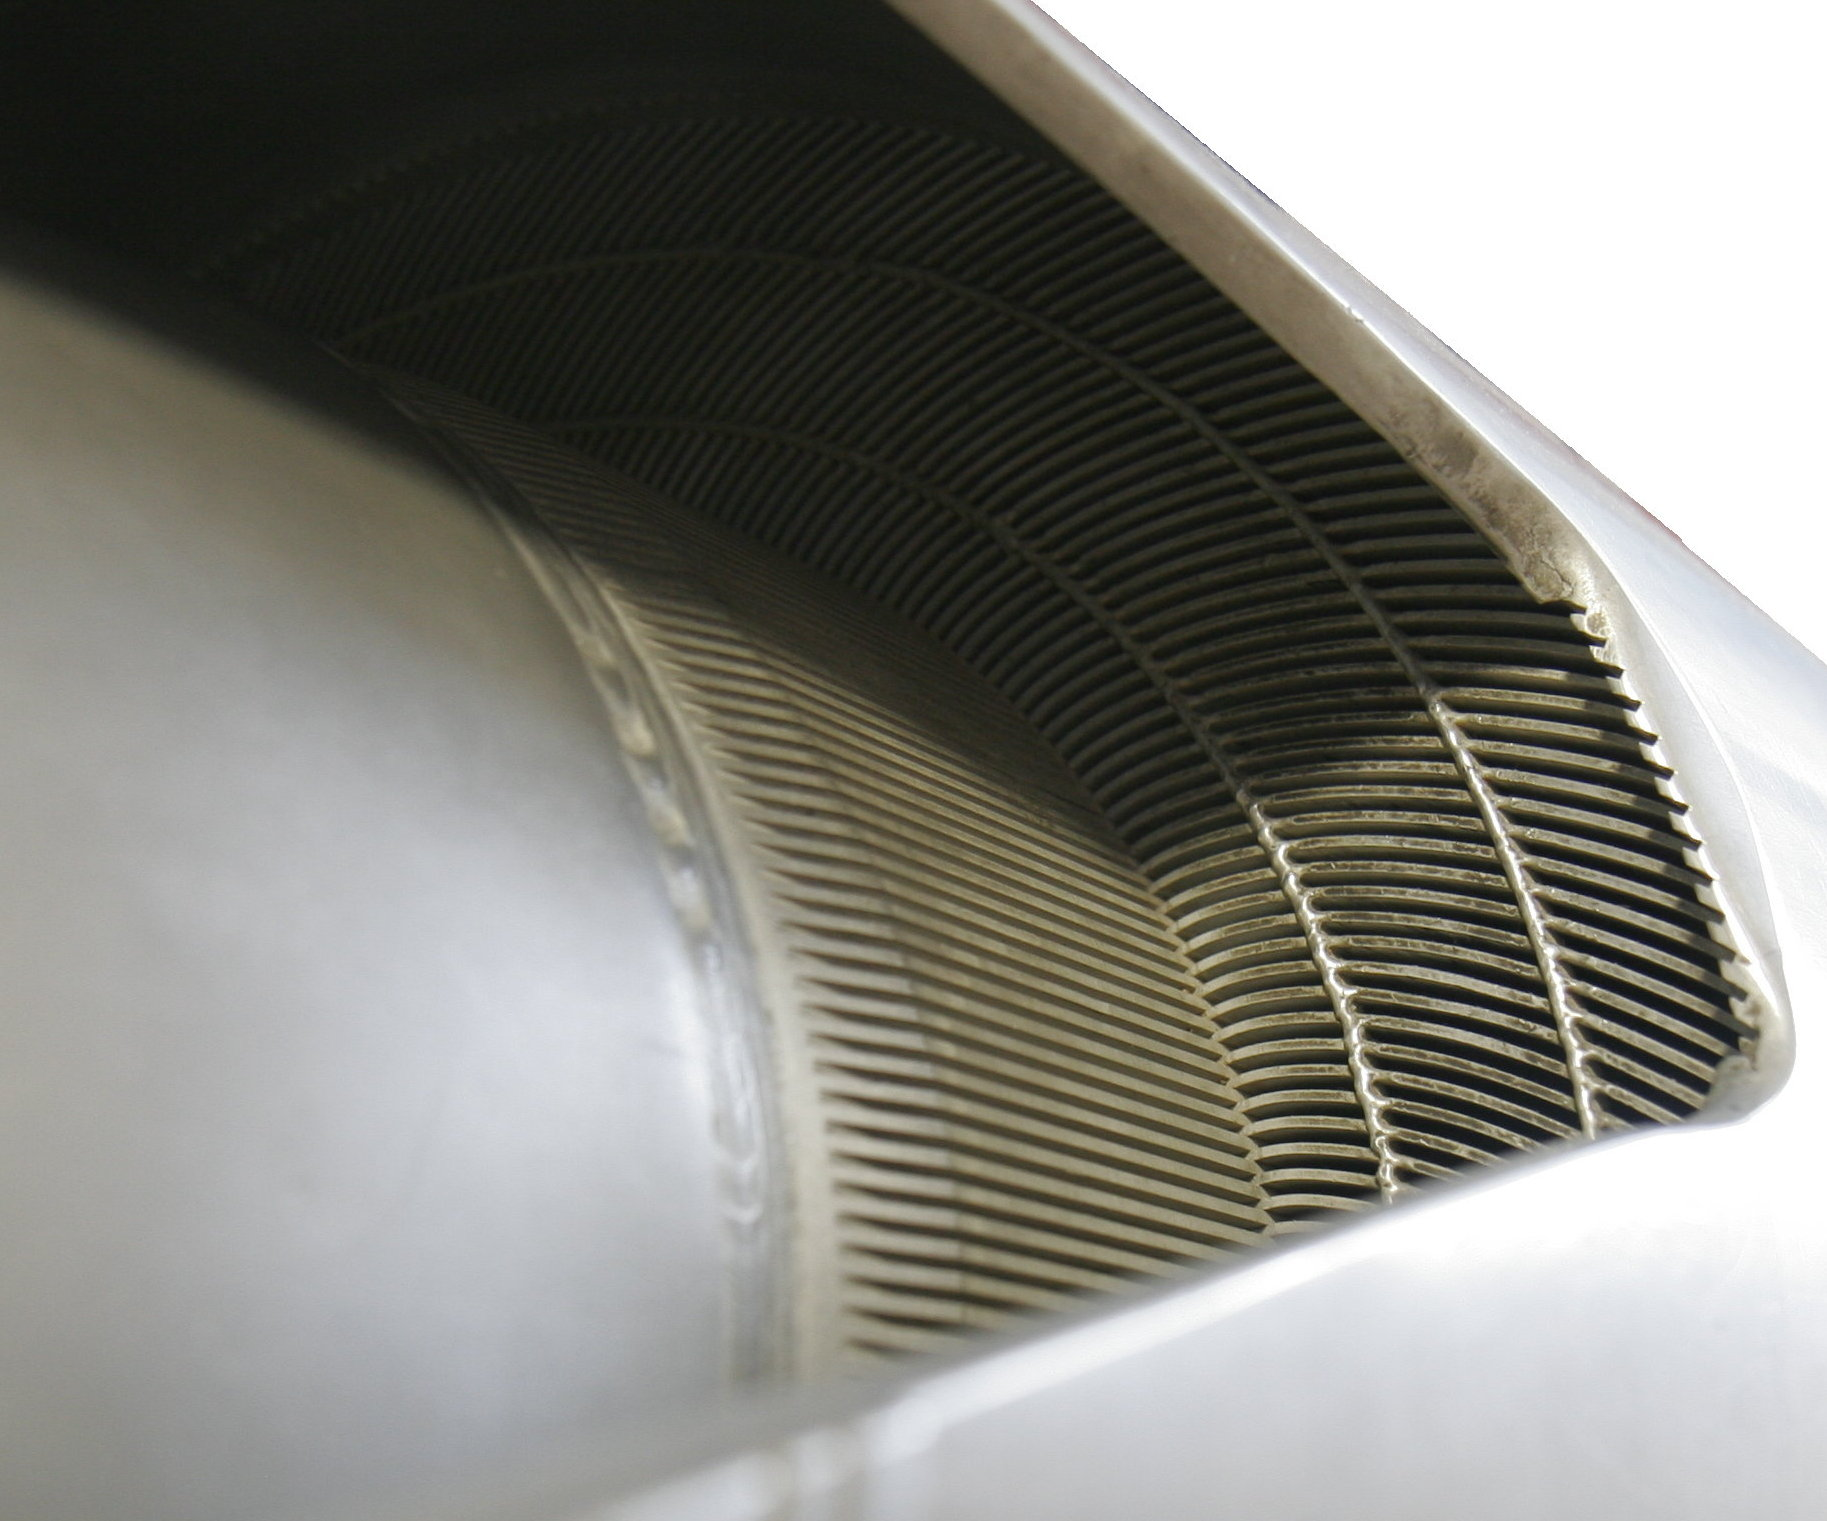
\includegraphics[width=0.8\linewidth]{images/ILL_core} 
\captionof{figure}[Coupe du support mécanique cylindrique de la cuve contenant le combustible fissible]{Coupe du support mécanique cylindrique de la cuve en aluminium laissant apparaitre le dessus des ailettes contenant le combustible. L'eau lourde circule par les fentes entre les ailettes. (source : \cite{ILL_core_8358_extract})} 
\label{fig:ill_core}
\end{figure}

} 

Les spécifications du réacteur de l'ILL sont un atout pour l'expérience \textsc{Stereo}. La forte teneur en $\ce{^{235}U}$ (93\% de fraction isotopique), offre une production d'antineutrinos provenant quasi exclusivement des produits de fission de cet isotope. En effet, en moyenne l'$\ce{^{235}U}$ contribue pour 99.3 \% du flux. Le reste est émis par le $\ce{^{239}Pu}$, lui-même formé pendant le cycle de fonctionnement par réactions successives à partir d'$\ce{^{238}U}$. Sa contribution s'élève à 0.7\% en moyenne sur un cycle. Cependant, il est important de noter qu'à basse énergie des corrections sur la prédiction des spectres antineutrinos émis sont nécessaires pour prendre en compte les neutrinos issus de la décroissance Beta de l'$\ce{^{28}Al}$. En effet, puisque la matrice combustible et la cuve d'eau lourde sont soumises à un haut flux de neutron, de nombreuses captures sur l'Aluminium ont lieu.\\ 

Un des atouts majeurs pour l'expérience \textsc{Stereo} est la compacité du combustible fissible. La géométrie du c\oe ur de l'ILL permet de mesurer des neutrinos avec une précision sur la distance de propagation allant jusqu'à $\pm \SI{20}{cm}$ $(1 \sigma)$, idéal pour mesurer des oscillations sur quelques mètres.\\ 

Le flux d'antineutrino émis peut être estimé à partir de la puissance thermique dégagée par le réacteur : 

\begin{equation} 
\label{eq:phi_nu_em} 
\phi_\nu^\textrm{em} \simeq \frac{\left<P_{th}\right>}{\left<E_{th}^{\textrm{fission}} (\ce{^{235}U})\right>} N_{\nu_e / \textrm{fission}}(\ce{^{235}U}), 
\end{equation} 

\bigbreak 

où $\left<P_{th}\right>$ est la puissance thermique mesurée en temps réel lorsque le réacteur est en fonctionnement, $\left<E_{th}^{\textrm{fission}} (\ce{^{235}U})\right>$ désigne l'énergie libérée par fission et $N_{\nu_e / \textrm{fission}}(\ce{^{235}U})$ est le nombre d'antineutrinos émis par fission. La puissance nominale du réacteur $\left<P_{th}\right>$ est de $\SI{58}{MW}$, et l'énergie libérée par fission d'Uranium 235 est de $\left<E_{th}^{\textrm{fission}} (\ce{^{235}U})\right> \simeq \SI{200}{MeV}$. En prenant le nombre moyen de neutrinos émis au-dessus du seuil en énergie de l'IBD, $N_{\nu_e / \textrm{fission}}(\ce{^{235}U}) \simeq 2$, l'ordre de grandeur du flux de neutrino peut être approché : 

\begin{equation} 
\phi_{\overline{\nu}_e} \simeq \SI{E18}{\overline{\nu}_e s^{-1}}. 
\end{equation} 

\bigbreak 

Ce chiffre peut paraître vertigineux, mais en incluant des considérations de sections efficaces de détection ainsi que d'angle solide et volume de détection, le nombre de neutrinos détectés est finalement de l'ordre de $\SI{400}{\overline{\nu}_e}$ par jour. Un calcul plus précis est présenté dans la section \ref{sec:nu_emission}. La composante dominante dans le bilan d'erreurs systématiques sur $\phi_{\overline{\nu}_e}$ est sur la mesure de la puissance thermique $\left<P_{th}\right>$. Néanmoins, l'instrumentation de l'ILL permet d'atteindre une bonne précision sur $P_{th}$ pour un réacteur de recherche et donc une mesure pertinente de la normalisation du flux de neutrinos.\\ 

Le réacteur de l'ILL alterne les périodes de fonctionnement (ON) et d'arrêt (OFF) par cycles d'environ 70 jours. Le réacteur génère ainsi des neutrinos pendant 3 cycles de 50 jours par an. Les périodes d'arrêt sont l'occasion de renouveler le combustible, et également d'effectuer divers travaux de maintenance dans le hall du réacteur. Ces périodes OFF offrent à \textsc{Stereo} la possibilité de mesurer les bruits de fond d'origine cosmique, élément essentiel à l'extraction du signal neutrino.\\ 

% Outre le fait que les mesures du spectre beta qui ont fournissent les prédictions des spectres neutrinos ont été effectuées sur ce réacteur, 

\subsection{Localisation de l'emplacement de Stereo : casemate PN3} 

La longueur d'oscillation vers un neutrino stérile pointée par la RAA est de l'ordre de quelques mètres à $\SI{1}{MeV}$. Le détecteur \textsc{Stereo} a été placé en conséquence avec une gamme de mesure de distance de propagation allant de 9.4 à 11.2 m, dans la casemate PN3 située dans le hall expérimental (voire figure \ref{fig:level_C_top_plan}). L'emplacement est surplombé par un canal d'eau qui permet le transfert et le stockage des combustibles usés. Le détecteur est placé dans l'alignement du canal afin de maximiser l'atténuation du flux de particules d'origine cosmique. Ce dernier permet de totaliser une épaisseur de blindage de $\SI{18}{m}$ équivalent eau \cite{LASSERRE201481}. Ainsi, le flux muonique est atténué d'un facteur 3 en moyenne selon l'angle d'incidence du muon \cite{docdb31}, un atout essentiel à toute expérience neutrino en surface. L'alignement de \textsc{Stereo} dans la direction du canal explique le décalage de 17.9 degrés entre l'axe du détecteur et celui du c\oe ur du réacteur, visible sur la figure \ref{fig:level_C_top_plan}.\\ 

\afterpage{ 

\begin{figure}[h!] 
\centering 
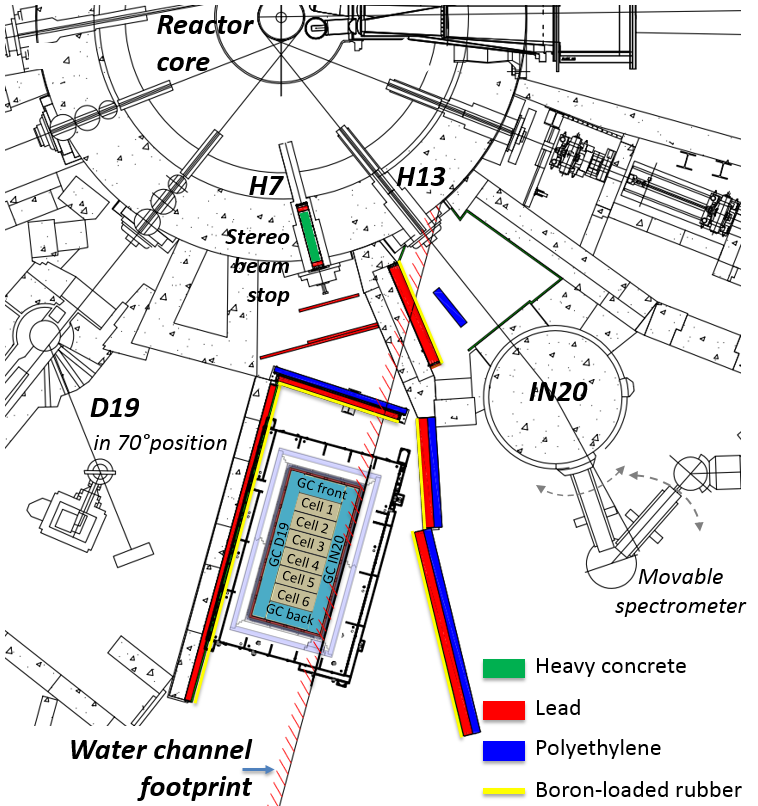
\includegraphics[width=0.8\linewidth]{images/level_C_top_plan} 
\caption[Plan du niveau C, centré sur la casemate de \textsc{Stereo}]{Plan du niveau C, centré sur la casemate de \textsc{Stereo}. Les différents blindages sont représentés en couleur et le bord du canal d'eau est délimité par la droite hachurée en rouge. L'angle entre la direction du détecteur et l'axe c\oe ur-centre du réacteur est de 17.9°. (source : \cite{Allemandou:2018vwb})} 
\label{fig:level_C_top_plan} 
\end{figure} 

} 

Malgré l'isolation spatiale de la casemate PN3, son environnement reste très bruité en radiations, notamment à cause de ses deux voisins D19 et IN20. Lorsque ces instruments sont en marche, ils génèrent un important bruit de fond de neutrons et de rayonnement gamma associés aux captures neutron sur les matériaux environnants. De plus, elles génèrent des champs magnétiques intenses qui peuvent affecter les photomultiplicateurs de \textsc{Stereo}. Pour concevoir les blindages adéquats, des études avancées sur les bruits de fond ont été entreprises pendant la phase de conception du détecteur. La nature des bruits de fond et les blindages employés seront détaillés dans la section suivante.\\ 

\subsection{Bruits de fond et blindages} 

La précision sur la mesure des spectres neutrino dépend non seulement de la quantité de neutrinos accumulée lors de la prise de données, mais aussi et surtout, de la nature et du taux de bruit de fond auquel est confronté le signal neutrino. Bien que la segmentation du détecteur et la capacité de discrimination du liquide scintillant permettent de rejeter les événements de bruit de fond en post-acquisition, l'utilisation de blindages adéquats reste vitale. Des campagnes de mesures dédiées ont été menées dans le but d'identifier la nature des bruits de fond, et de concevoir les blindages à ériger.\\ 

\subsubsection*{L'environnement de la casemate} 

Les sorties des tubes de faisceau H7 et H13 ainsi que le faisceau de D19 sont des sources importantes de bruit de fond gamma, neutrons rapides et thermiques. En effet, ces tubes prélèvent les neutrons directement depuis le c\oe ur pour les amener hors du blindage réacteur. En principe, ces lignes sont employées par les instruments qui se servent des faisceaux de neutrons pour irradier une cible. La sortie H7, normalement destinée à PN3, a été obstruée par un bouchon constitué de plusieurs matériaux : polyéthylène boré, plomb et béton lourd. La ligne H13 quant à elle est toujours en service pour IN20. Afin d'atténuer au maximum le flux de neutrons et gammas induits par ces tubes, des murs en plomb et polyéthylène ont été construits autour du détecteur \textsc{Stereo}.\\ 

Les instruments disposés dans les emplacements D19 et IN20 sont aussi des sources importantes de bruit de fond gamma. De plus, leurs spectres d'émission et leurs taux de comptage varient très fortement dans le temps puisque leurs conditions expérimentales sont constamment ajustées : nature des cibles, orientation des spectromètres ou encore intensité du faisceau neutron. Pour réduire davantage le taux de bruits de fond sur le signal neutrino, les murs délimitant la casemate PN3 ont été renforcés par des couches de plomb et de polyéthylène jusqu'à une hauteur de $\SI{2.4}{m}$. Ces blindages sont représentés en couleurs sur la figure \ref{fig:level_C_top_plan}.\\ 

L'expérience IN20 exploite aussi des champs magnétiques très intenses (jusqu'à $\SI{15}{T}$) dont les fuites de champ s'étendent jusque dans la casemate à hauteur de quelques centaines de $\mu T$,soit plusieurs fois la valeur du champ terrestre, et dans des directions variant avec l'orientation de l'aimant. De tels champs magnétiques affectent la stabilité du gain des photomultiplicateurs, c'est pour cette raison qu'un blindage magnétique a été déployé autour du détecteur.\\ 

\subsubsection*{Les blindages autour du détecteur} 

Malgré l'isolation de la casemate, des neutrons et gammas sont toujours présents. Afin de réduire les bruits de fond atteignant le volume cible, le détecteur est placé au c\oe ur d'une poupée russe de blindages. Une couche de polyéthylène boré entoure le détecteur interne avec une épaisseur de $\SI{29}{cm}$ en haut pour atténuer les neutrons verticaux induits par les cosmiques dans le canal d'eau, $\SI{20}{cm}$ au fond pour les neutrons cosmogéniques créés dans le sol, et $\SI{15}{cm}$ sur les côtés. Celui-ci permet la thermalisation puis la capture des neutrons qui le pénètrent, sans émettre de nouveaux gammas. Autour de ce dernier se place une épaisseur de plomb de $\SI{20}{cm}$ en bas pour arrêter les gammas de décroissance de l'isotope $\ce{^{16}N}$ provenant du circuit primaire qui passe en dessous du détecteur\footnote{Cet $\ce{^{16}N}$ provient de l'activation de $\ce{^{16}O}$ de l'eau lourde quand elle passe dans le c\oe ur: $\ce{^{16}O} + n \rightarrow \ce{^{16}N^*} + p$ ; $\ce{^{16}N^*} \rightarrow \ce{^{16}N} + \gamma(\SI{6}{MeV})$.}, $\SI{15}{cm}$ au plafond pour atténuer l'ambiance gamma qui vient par le haut du détecteur, et $\SI{10}{cm}$ pour les murs verticaux. Le tout est maintenu par une armature en poutres métalliques, qualifiée antisismique, comme le montre la photo Figure \ref{fig:photos_blindages_stereo}. Le champ magnétique est atténué grâce à un revêtement en fer doux d'$\SI{1}{cm}$ autour la structure métallique et $\SI{1,5}{mm}$ autour du détecteur interne, ainsi que des cylindres de même matière disposés autour de chaque photomultiplicateur. Enfin, chaque paroi est recouverte par des plaques de caoutchouc chargé de bore pour capturer les neutrons thermiques ambiants. L'ensemble du blindage totalise une charge au sol de $\SI{93}{T}$, satisfaisant les contraintes de poids maximal de la casemate: $\SI{10}{T/m^2}$.\\ 

\afterpage{ 

\begin{figure}[h!] 
\centering 
\begin{subfigure}[b]{1\textwidth} 
\centering 
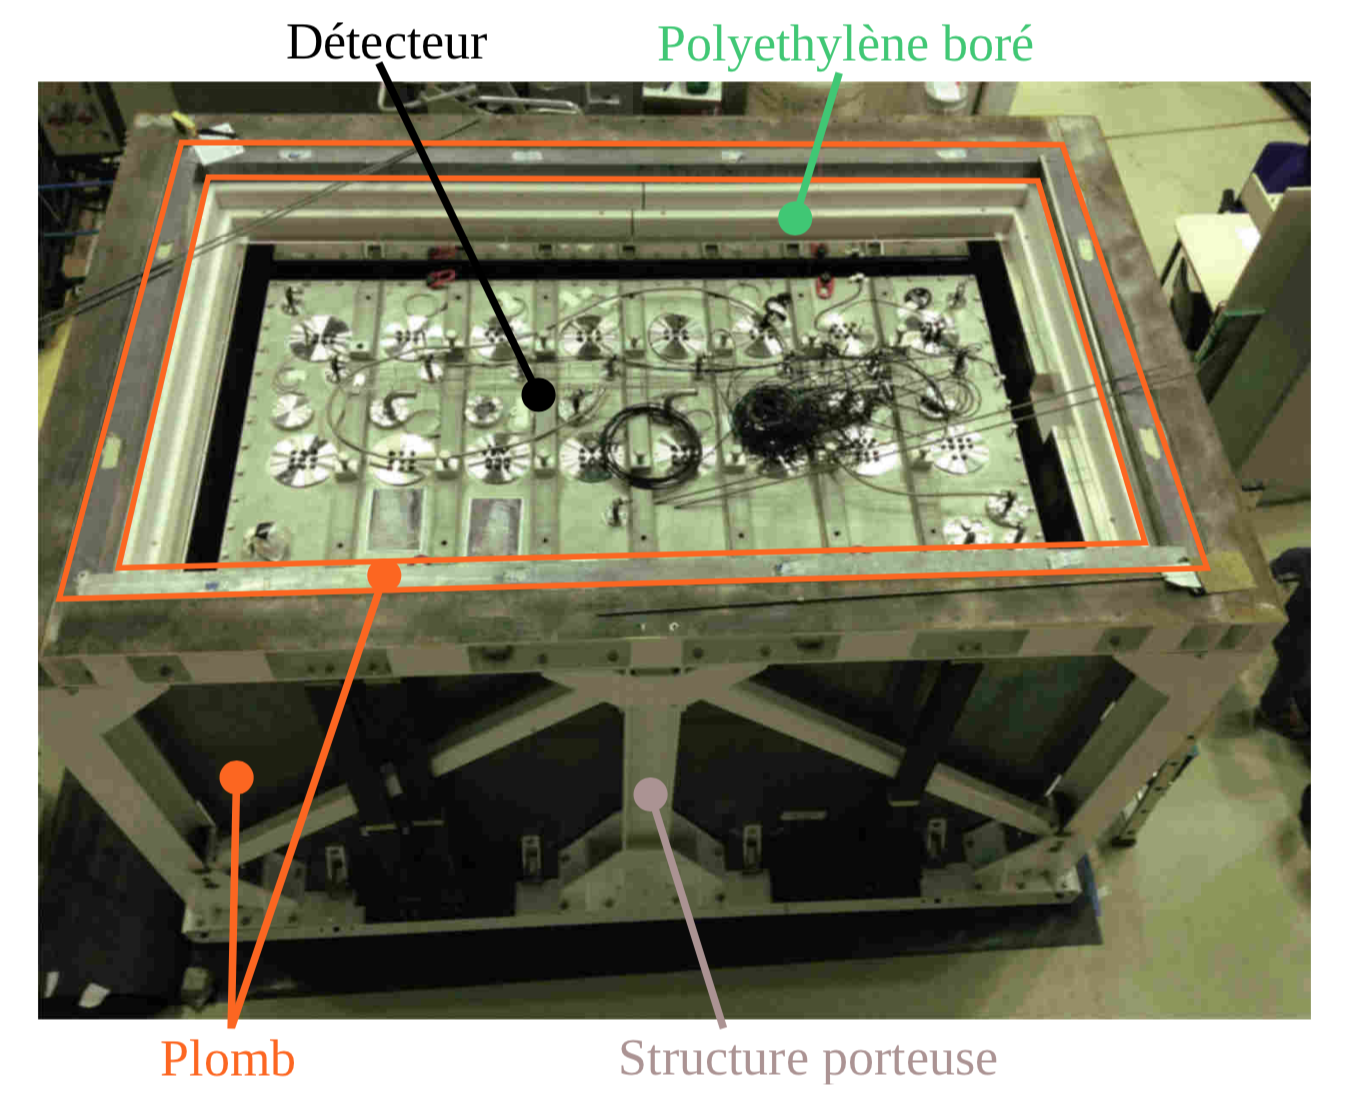
\includegraphics[width=0.8\linewidth]{images/blindages_internes.png} 
\caption{Vue du détecteur et des blindages insérés dans la structure porteuse.} 
\label{fig:blindages_internes.png} 
\end{subfigure} 
~ % attention ! space sensitive 
\begin{subfigure}[b]{1\textwidth} 
\centering 
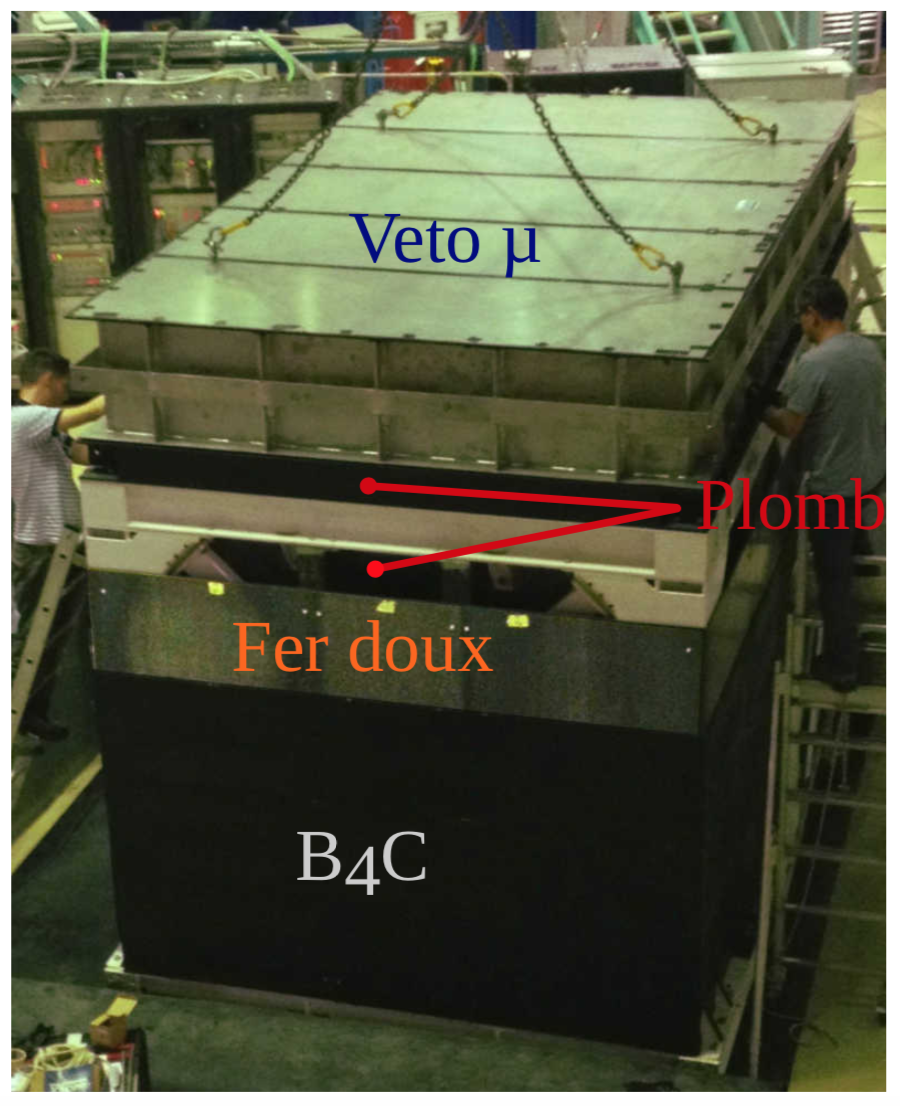
\includegraphics[width=0.55\linewidth]{images/blindage_externes.png} 
\caption{Photo des blindages superficiels autour la structure porteuse prise lors de l'installation du détecteur sur site.} 
\label{fig:blindage_externes.png} 
\end{subfigure} 
\caption[Photos des blindages entourant le détecteur.]{Photos des blindages entourant le détecteur. (source : \cite{bonhomme:tel-01931309})} 
\label{fig:photos_blindages_stereo} 
\end{figure} 

\clearpage 

} 

\subsubsection*{Le veto à muons} 

Bien que la présence de la piscine de stockage atténue grandement le flux de radiations d'origine cosmique, celui-ci reste trop important pour être ignoré. Un détecteur à rayonnement Cherenkov a été placé au-dessus du détecteur: c'est le veto muon. Il est constitué d'une cuve en acier inoxydable recouvrant toute la surface du détecteur, blindages compris. La cuve possède des parois réfléchissantes (Tyvek) et est remplie de $\SI{25}{cm}$ d'eau, contenant un additif (4- Methylumbelliferone) qui décale la longueur d'onde des photons émis par effet Cherenkov. La lumière est colletée par 20 photomultiplicateurs placés au-dessus de la surface de l'eau.\\ 

Le veto muon a pour fonction de signaler le passage d'un muon proche du détecteur interne. Les muons peuvent créer des neutrons rapides par spallation sur les noyaux composant le blindage, en particulier sur les noyaux lourds tels que le plomb. Ces neutrons peuvent être détectés et imiter parfaitement un signal neutrino. En pratique, c'est la composante de bruit de fond la plus importante dans \textsc{Stereo}.\\ 

%\begin{itemize} 
% \item Bruit de fond accidentel / IN20 D19 neutron gamma 
% \item neutron rapides H7 
% \item neutron env / Argon activé, capture sur Fe ou Al 
% \item mesure Bdf germanium (Anne ?) 
% \item bruit de fond cosmique / canal eau 
%\end{itemize} 
% 

%\begin{itemize} 

% \item Blindages passifs (Pb, B4C, polyéthylène, mu métal, fer doux) 

% \item Photos 

% \item Blindages actifs : Veto muons / GC 

%\end{itemize} 



\bigbreak 


\section{Principe de Détection} 

\subsection{Décroissance Beta inverse} 

Les antineutrinos sont détectés en interagissant dans le liquide scintillateur par décroissance Beta inverse (IBD). Cette réaction présente des avantages expérimentaux tels que : une section efficace plus élevée que le courant neutre, quadratique avec l'énergie du neutrino incident ($\sigma_{IBD} \propto G_F^2E_{\overline{\nu}_e}^2$), et connue avec une bonne précision; le fait que les liquides scintillants soient pourvoyeurs de protons libres; les produits de la réaction peuvent être identifiés distinctement, réduisant ainsi le bruit de fond drastiquement; ou encore la forte corrélation entre l'énergie du neutrino et celle du positron. Il n'est donc pas surprenant que l'IBD soit un des canaux de détection des neutrinos les plus utilisés depuis la découverte du neutrino.\\ 

La réaction correspond à l'interaction d'un antineutrino électronique avec un proton qui donne naissance à un positron et un neutron : 

\begin{equation} 
\ce{\overline{\nu}_e + p \rightarrow e^+ + n}. 
\end{equation} 

\bigbreak 

C'est une réaction à seuil en énergie, car la masse du proton est inférieure à la somme des masses du neutron et du positron: 

\begin{equation} 
E_{\overline{\nu}_e} > \SI{1.806}{MeV} \simeq m(n) + m(e^+) - m(p). 
\end{equation} 

\bigbreak 

Le principe de détection de \textsc{Stereo} repose sur la double identification positron-neutron corrélée en temps. Celui-ci se décompose en deux étapes: détection du positron (signal Prompt), et détection du neutron (signal Retardé). 

\bigbreak 

\subsubsection*{La détection du positron (Prompt)} 

Une fois émis, le positron ralentit en interagissant avec les molécules du liquide scintillateur tout comme un électron : par ionisation, rayonnement de freinage ou encore par excitation moléculaire qui est responsable de la production de lumière. En fin de parcours cependant, il s'annihile avec un électron du milieu pour donner naissance à deux gammas de $\SI{511}{keV}$. À cette énergie les gammas interagissent principalement par effet Compton ou effet photoélectrique, générant à leur tour des électrons de quelques keV. Ce processus se déroule dans une fenêtre de quelques centaines de picosecondes, une échelle en temps considérée comme instantanée au regard du système d'acquisition. La détection du positron est donc appelée événement \og Prompt \fg{}.\\ 

L'énergie cinétique du neutrino est très majoritairement transmise au positron \cite{Strumia:2003zx}. En effet, puisque sa masse est largement inférieure à celle du neutron, le positron emporte l'énergie cinétique et le neutron récupère la direction de l'impulsion. En définitive, l'énergie du neutrino est directement déduite de l'énergie déposée par le positron en appliquant un offset : $E_{\overline{\nu}_e} = E_{e^+}^{\textrm{dep}} + \SI{1.806}{MeV} - \SI{1.022}{MeV} = E_{e^+}^{\textrm{dep}} + \SI{0.784}{MeV}$, où $\SI{1.806}{MeV}$ est le seuil en énergie de la réaction IBD et $\SI{1.022}{MeV}$ est l'énergie déposée par les deux gammas issus de l'annihilation $e^+e^-$. \\ 

% Je pense qu'il y a juste à dire que: 
% * le rapport de masse Mn/Me fait que toute l'énergie cinétique du neutrino se retrouve dans celle du positron 
% * L’annihilation du positron compense 1.022 MeV par rapport au défaut de masse de l'IBD, d'où l'offset de 1.806-1.022 = 0.784 MeV. 

\subsubsection*{La détection du neutron (Delayed)} 

Dans la réaction IBD, le neutron n'emporte en moyenne qu'une dizaine de keV d'énergie cinétique. Il ralentit en collisionnant avec les noyaux du milieu jusqu'à thermalisation. Cette phase ne prend en moyenne que 5 microsecondes \cite{docdb746}. Ensuite, le neutron diffuse par chocs élastiques jusqu'à absorption. La phase de thermalisation n'est pas détectable en elle-même, c'est pourquoi \textsc{Stereo} exploite les propriétés de capture neutronique du gadolinium.\\ 

Bien que l'Hydrogène soit le noyau capturant les neutrons le plus abondant dans le liquide scintillateur, le volume de la cible a été dopé avec du gadolinium pour maximiser le rapport signal sur bruit via deux facteurs. Le premier concerne la minimisation du temps de capture. Le temps de capture des neutrons s'exprime comme une fonction de leur vitesse moyenne $\left<v\right>$ et de leur distance moyenne parcourue sans interaction $\lambda$ avec un noyau absorbant. Puisqu'ils sont thermalisés, la distribution des vitesses suit une loi de Maxwell-Boltzmann et la vitesse moyenne peut être exprimée comme une fonction de la température du liquide $k_BT$. La distance moyenne parcourue quant à elle est directement liée à la section efficace de capture $\sigma_{n-X}$ et la densité de noyaux absorbants $n_{X}$. Le temps de capture neutron sur un noyau X s'écrit :\\ 

\begin{equation} 
\label{eq:neutron_capture_time} 
\tau_{n-X} = \frac{\lambda_n}{\left<v\right>} = \frac{1}{n_{X}\sigma_{n-X}} \sqrt{\frac{m_n}{3 k_B T}}.
\end{equation} 

\bigbreak 

L'Hydrogène a une section efficace de l'ordre du barn alors que celle des noyaux de gadolinium ($\ce{^{155}Gd}$ et $\ce{^{157}Gd}$) atteint quelques centaines de milliers de barns. En dopant le liquide scintillateur à hauteur de 0.2 \% de la masse, le temps de capture moyen est réduit à $\SI{16}{\mu s}$ contre $\SI{230}{\mu s}$ avec uniquement l'Hydrogène.\\ 

Le second facteur concerne l'énergie des gammas de désexcitation. L'absorption d'un neutron affecte la structure interne du noyau et la désexcitation de ce dernier conduit à l'émission d'un ou plusieurs gammas. L'énergie et le nombre de gammas émis dépendent des niveaux sollicités lors de la désexcitation. Dans le cas de l'Hydrogène un seul gamma est émis avec une énergie de $\SI{2.2}{MeV}$, alors que les noyaux de gadolinium génèrent plusieurs gammas en cascade dont la somme de leurs énergies totalise environ $\SI{8}{MeV}$. La détection de ces gammas de désexcitation nucléaire est baptisée événement \og Retardé \fg{}. Afin de réduire au maximum le nombre de coïncidences fortuites, l'identification de ces gammas doit être effectuée dans une fenêtre en énergie où le bruit de fond est au plus bas. Or, les gammas de la radioactivité naturelle ne dépassent pas l'énergie de 2.6 MeV. La signature gamma du gadolinium est donc un candidat de choix pour signer la présence d'un neutron.\\ 

Cependant, les cascades gamma du gadolinium présentent quelques difficultés supplémentaires en simulation. En effet, la multiplicité des gammas émis augmente l'extension spatiale des dépôts d'énergie, y compris dans des matériaux non scintillants. De plus, les niveaux de désexcitation des noyaux de gadolinium ne sont pas connus jusqu'à $\SI{8}{MeV}$. Une étude approfondie sur la génération des gammas de cascade a été menée, et a fait l'objet d'une publication \cite{AlmazanMolina:2019aoc}. Ces aspects sont détaillés dans la section \ref{sec:cascade_Gd_MC}.\\ 

\bigbreak 

\subsection{Processus de scintillation} 
\label{seq:scintillation} 

Le mécanisme qui convertit les dépôts d'énergie cinétique en photons du spectre visible est appelé \og processus de scintillation \fg{}. Il existe plusieurs types de matériaux scintillateurs qui exploitent des propriétés de fluorescence différentes, et chacun d'eux a ses propres caractéristiques : temps de réponse, rendement lumineux, contraintes de fabrication. Les matériaux choisis dans \textsc{Stereo} sont sous forme de liquide organique.\\ 

Microscopiquement parlant, l'énergie cinétique est transmise par les particules libres et chargées qui traversent le milieu. Ces dépôts d'énergie se font par ionisation, rayonnement de freinage ou excitation des molécules environnantes. C'est l'excitation moléculaire qui est responsable de la scintillation. En effet, la désexcitation des liaisons $\pi$ des molécules organiques produit des photons optiques \cite{Birks:1964zz}. Les photons sont générés par la dernière transition sur des états singulets ($S_x$) : $S_1 \rightarrow S_0$ où $S_0$ est l'état fondamental. Les états vibrationnels, qui forment une structure fine autour des états $S_1$ et $S_0$, permettent de rendre le milieu transparent à sa propre lumière. En effet, l'énergie des photons émis entre $S_1$ et $S_0 + \delta$ n'est pas suffisante pour induire de nouveau $S_0 \rightarrow S_1$.\\ 

Le processus de scintillation peut être parfois retardé. L'interaction des particules chargées avec les molécules peut aussi exciter les liaisons $\pi$ sur des états triplets ($T_x$). Dans ce cas, le mécanisme de désexcitation ($T_x \rightarrow T_0$) se produit sans émettre de photons. En revanche, l'interaction de deux molécules sur $T_0$ à proximité l'une de l'autre convertit les états des molécules : $T_0 + T_0 \rightarrow S_x + S_0 + P$ où $P$ est une quantité d'énergie dissipée sous forme de vibrations (phonons). La molécule sous $S_x$ génère des photons de scintillation comme il a été décrit précédemment. Le temps caractéristique de scintillation est cette fois de quelques dizaines de nanosecondes et la lumière générée est donc retardée. Cette composante devient significative lorsque la densité des dépôts d'énergie est trop importante. C'est le cas des neutrons rapides qui induisent par collision des protons de recul avec un fort pouvoir d'arrêt ($dE/dx$) en fin de parcours et déposent donc beaucoup d'énergie dans une zone localisée. Ainsi, la composante lumineuse retardée est significativement plus élevée pour les neutrons rapides que pour les électrons. Cette différence est mesurable en analysant la forme des pulses des photomultiplicateurs. La méthode de discrimination en forme des signaux (aussi appelé \textit{PSD} pour \textit{Pulse Shape Discrimination}) est présentée plus en détail dans la section \ref{sec:PSD_principe}.\\ 

Un autre effet qui se manifeste lorsque les dépôts d'énergie sont trop denses est le quenching. À partir d'un certaine densité de molécules excitées, le rendement lumineux diminue, car les cortèges électroniques commencent à interagir entre eux, altérant le processus de scintillation. Lorsque les particules ionisantes ont suffisamment ralenti, leur pouvoir d'arrêt ($dE/dx$) augmente fortement \cite{PDG_particle_matter_2018}. Cela signifie qu'elles déposent toute leur énergie dans une région localisée. Pour des électrons de plus de $\SI{400}{keV}$, la fraction d'énergie qui a saturé le pouvoir de scintillation est négligeable; la réponse en photons est linéaire avec l'énergie. En deçà de ce seuil, le rendement lumineux diminue significativement. En pratique, des gammas sont utilisés pour calibrer la réponse du détecteur. Leurs interactions avec le liquide scintillateur génère des électrons Compton qui engendrent la création de photons optiques. Par rapport aux électrons, l'effet de quenching des gammas se manifeste donc à une énergie plus haute. Un modèle effectif de quenching a donc été implémenté et ajusté dans la simulation afin de reproduire les non-linéarités du processus de scintillation. Cette étude est présentée dans la section \ref{sec:quenching}.\\ 

La production de lumière par effet Tcherenkov contribue aussi au processus de scintillation. En effet, lorsqu'une particule chargée traverse un milieu à une vitesse plus grande que celle de la lumière\footnote{Les photons voyagent toujours à la vitesse $c$. Cependant dans certains milieux, l'interaction d'une onde électromagnétique avec les électrons fait que les molécules agissent comme des dipôles. Le mouvement collectif des électrons créé une nouvelle onde qui interfère avec l'onde originale et dont la résultante a une vitesse de phase inférieure à la vitesse de la lumière dans le vide \cite{doi:10.1119/1.12596}.}, celle-ci provoque l'émission de photons dont la direction de propagation est dirigée suivant un angle $\theta$ respectant la relation : 

\begin{equation} 
\textrm{cos}(\theta ) = 1 / (\beta n),
\end{equation} 

\bigbreak 

où $\beta$ est le rapport de la vitesse de la particule sur celle de la lumière dans le vide, et $n$ l'indice optique du milieu \cite{Cerenkov:1937vh}. La quantité d'énergie rayonnée par unité de longueur parcourue par la particule incidente suit la relation de proportionnalité \cite{Frank:1937fk} : 

\begin{equation} 
dE \propto \left(1 - \frac{1}{\beta^2n^2} \right).
\end{equation} 

\bigbreak 

L'énergie seuil est telle que $\beta_{th} > 1/n$. En utilisant $E = \gamma mc^2$, où $\gamma$ est le facteur de Lorentz, l'énergie seuil s'écrit finalement : 

\begin{equation} 
E_{th} = \frac{mc^2}{\sqrt{1 - \frac{1}{n^2}}}.
\end{equation} 

Pour des électrons, l'énergie cinétique seuil est d'environ $\SI{200}{keV}$ en considérant l'indice optique du liquide à $n \sim 1,5$ pour la lumière visible. Le nombre de photons émis sur une distance $l$ et dans une région spectrale confinée entre $\lambda_1$ et $\lambda_2$ peut être calculé avec: 

\begin{equation} 
N_\gamma = 2\pi \alpha l \left(\frac{1}{\lambda_2} - \frac{1}{\lambda_1} \right) \left( 1 - \frac{1}{\beta^2n^2} \right),
\end{equation} 

\bigbreak 

où $\alpha = 1/137$ est la constante de structure fine. En prenant arbitrairement $\lambda_1 = \SI{350}{nm}$ et $\lambda_2 = \SI{450}{nm}$\footnote{Ces longueurs d'onde correspondent à la bande passante où l'efficacité quantique des photomultiplicateurs est maximale \cite{Wang:2015vla}.}, le nombre de photons émis atteint rapidement un plateau à $N_\gamma \sim 150$ par cm pour des électrons d'énergie cinétique supérieure à $3 \SI{}{MeV}$ (voire figure \ref{fig:Cerenkov_radiation_electron.pdf}).\\ 

\afterpage{ 

\begin{figure}[h!] 
\centering 
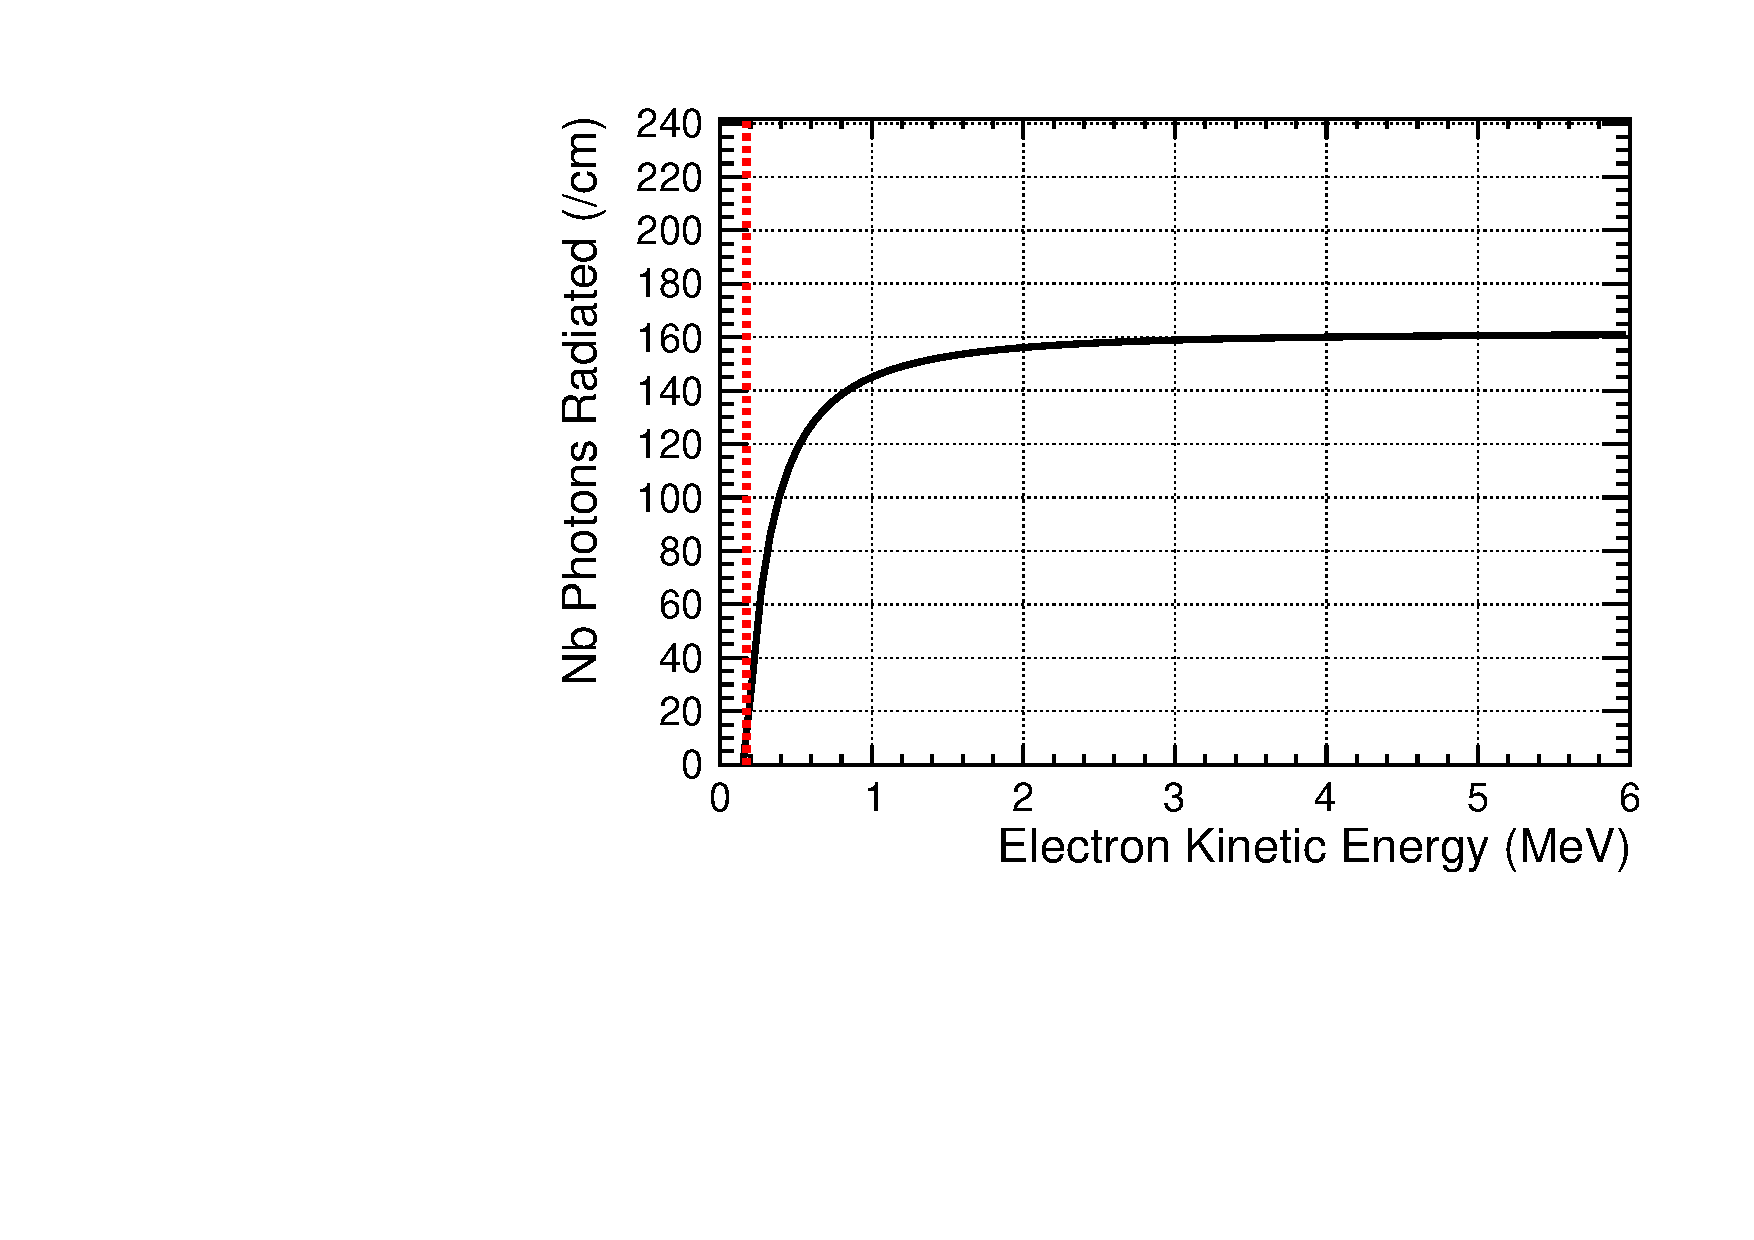
\includegraphics[width=0.9\linewidth]{images/Cerenkov_radiation_electron.pdf} 
\caption[Nombre de photons rayonnés par effets Tcherenkov en fonction de l'énergie cinétique de l'électron.]{Nombre de photons rayonnés par effets Tcherenkov pour un électron parcourant $\SI{1}{cm}$ dans le liquide. Dans cet exemple, l'indice optique a été choisi à $n \sim 1,5$, et la bande passante de photons optiques : $\SI{350}{nm} < \lambda < \SI{450}{nm}$. La ligne rouge représente l'énergie cinétique seuil pour cet effet.} 
\label{fig:Cerenkov_radiation_electron.pdf} 
\end{figure} 

} 


Bien que le processus de scintillation soit largement dominé par les molécules organiques ($\sim \SI{7000}{photons/MeV}$), l'effet Tcherenkov est aussi pris en compte dans la simulation. 

\bigbreak 

% 511/sqrt(1 - 1/(1.5*1.5)) - 511 
% e pense qu'il faut aborder ce point succintement: 
% * La production de lumière Cerenkov a aussi lieu puisque le seuil pour un électron dans le liquide vaut XX keV. 
% * Donner un exemple de fraction de lumi!re Cerenkov par rapport à la scintillation (quelques % pour un e- de 5 MeV) 
% * Le processus est bien-sur inclu dans la simulation. 

\bigbreak 

\section{Le détecteur \textsc{Stereo}} 

\subsection{Le détecteur interne} 

Le détecteur interne a été conçu et construit par le CEA-Saclay. Le volume cible où interagissent les neutrinos est délimité pas un aquarium avec des parois en acrylique de $\SI{12}{mm}$ d'épaisseur, dont la surface au sol fait $\SI{913}{mm}$ de large contre $\SI{2232}{mm}$ de long. Il contient le liquide scintillateur dopé au gadolinium qui s'élève à hauteur de $\SI{918}{mm}$. Ce volume est nommé \og \textit{Target} \fg{}. Il est segmenté dans le sens de la longueur en 6 cellules identiques séparées par des plaques en acrylique de $\SI{4}{mm}$ d'épaisseur. Chaque cellule a le même volume de liquide scintillateur ($368 \times 889 \times 918 \ \SI{}{mm^3}$), mais couvre une distance de propagation neutrino différente (voire Figure \ref{fig:Propagation_Lenghts.pdf} et Tableau \ref{tab:propagation_lenghts}).\\ 

\afterpage{ 

\begin{figure}[h!] 
\centering 
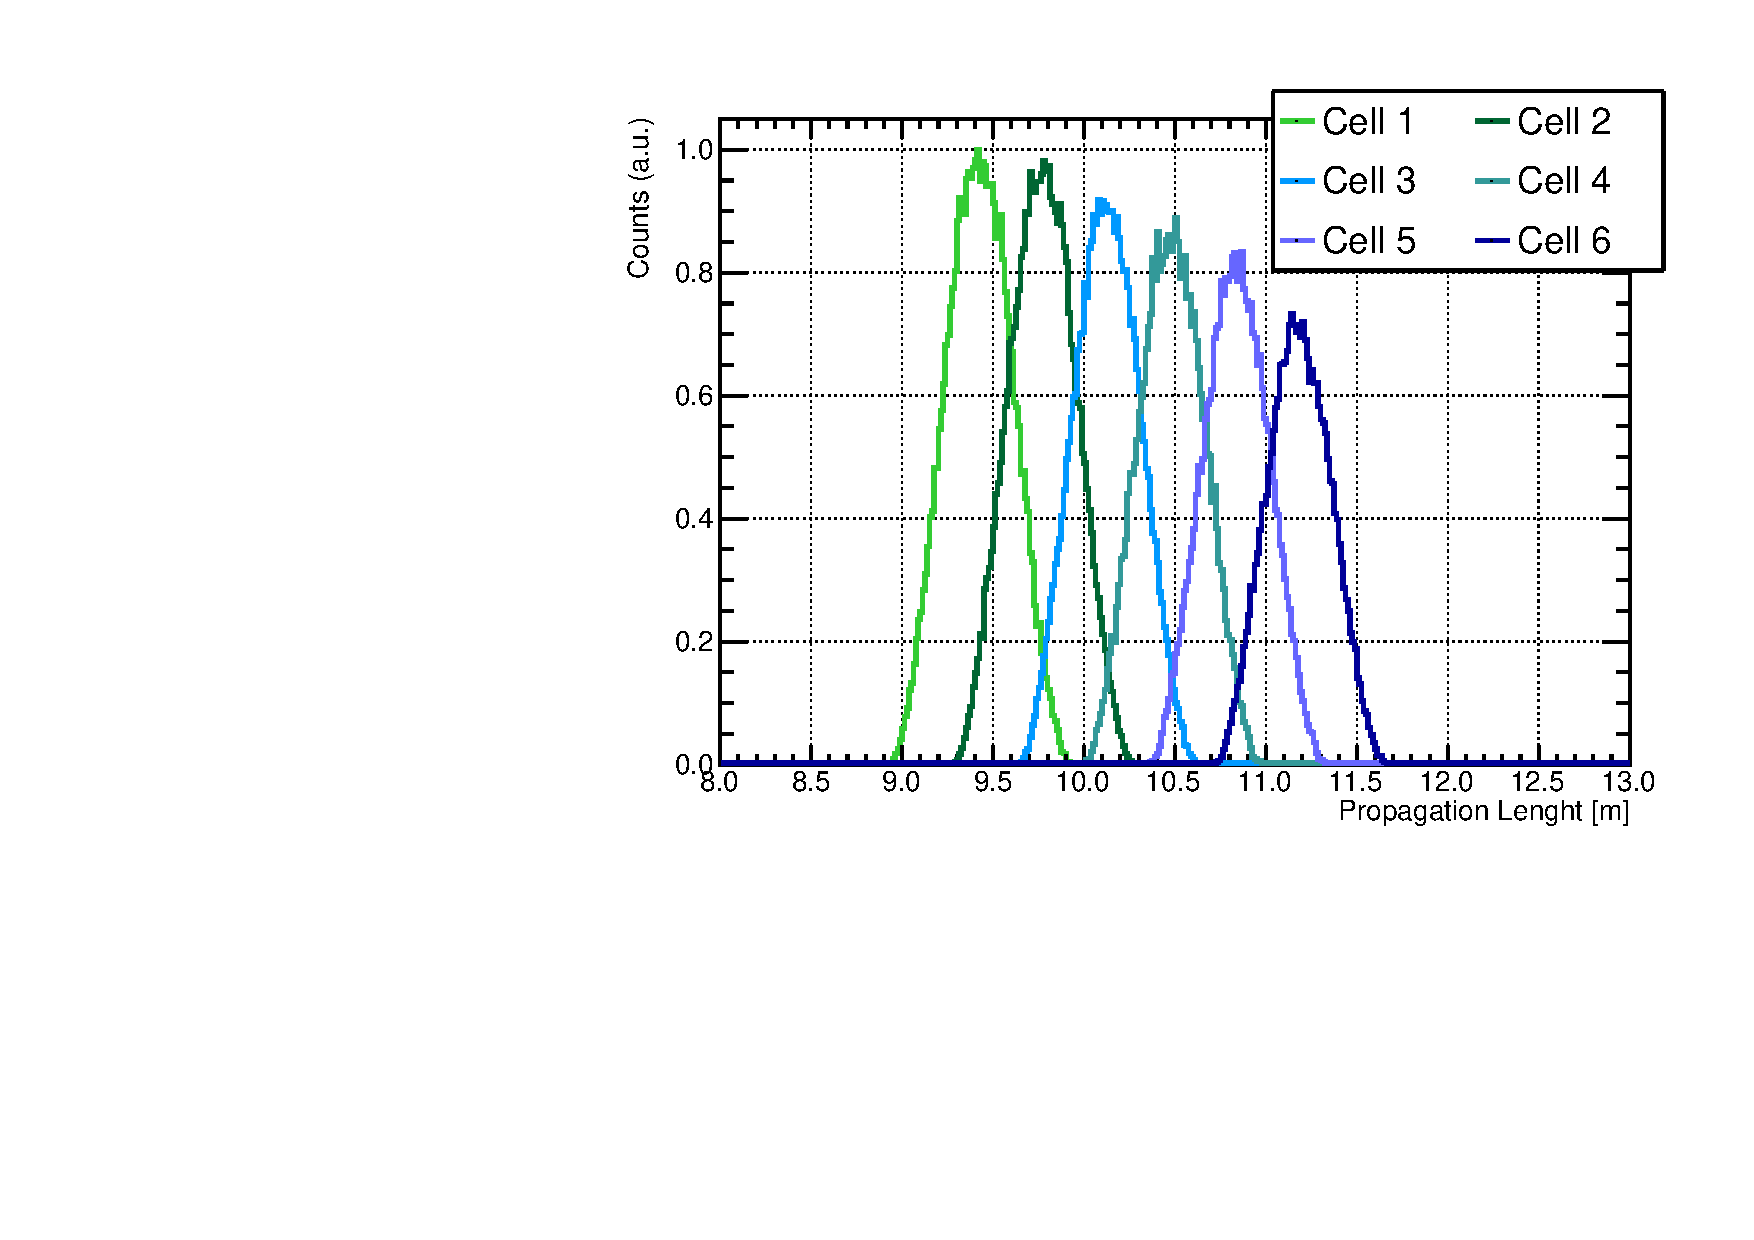
\includegraphics[width=0.94\linewidth]{images/Propagation_Lenghts.pdf} 
\caption[Distances de propagation couvertes par les six cellules de la Target]{Distances de propagations couvertes par les 6 cellules de la Target. L'effet de l'angle solide de chaque cellule sur le taux de neutrinos attendu est ici inclus: d'où l'allure décroissante en fonction des cellules.} 
\label{fig:Propagation_Lenghts.pdf} 
\end{figure} 

\begin{table}[h!] 
\begin{center} 
\begin{tabular}{|c|c|c|} 
\hline 
Cellule & Distance de propagation moyenne (m) & Variance (m)\\ 
\hline 
1 & 9,42 & 0,18\\ 
\hline 
2 & 9,77 & 0,18\\ 
\hline 
3 & 10,13 & 0,18\\ 
\hline 
4 & 10,48 & 0,18\\ 
\hline 
5 & 10,84 & 0,17\\ 
\hline 
6 & 11,18 & 0,17\\ 
\hline 
\end{tabular} 
\captionof{table}{Liste des distances de propagations moyennes des neutrinos par cellule.} 
\label{tab:propagation_lenghts} 
\end{center} 
\end{table} 

} 

La Target est entourée par une couronne de liquide scintillateur sans gadolinium appelée \og \textit{Gamma-Catcher} \fg{}. Sa fonction principale est de récupérer les fuites d'énergie des gammas émis par l'annihilation du positron (signal Prompt) et ceux de la cascade gamma du gadolinium. Le Gamma Catcher permet aussi d'agir comme un blindage actif contre les rayonnements provenant de l'extérieur. Cette couronne est divisée en 4 sous-volumes, dont deux qui ont la même géométrie que les 6 cellules --- appelés \og \textit{Short Gamma Catcher Cells} \fg{} --- et qui sont placés en prolongement de la Target (une devant la cellule 1 et une derrière la cellule 6) pour minimiser les effets de bord en rajoutant des cellules de géométries identiques devant et derrière, et les deux autres qui couvrent toute la longueur du détecteur sont baptisées \og \textit{Long Gamma Catcher Cells} \fg{}. L'ensemble en acrylique est placé dans une double cuve en acier inoxydable qui solidifie la structure et prévient des éventuelles fuites de liquide scintillateur.\\ 

Les 48 photomultiplicateurs (PMs) sont placés au-dessus de chaque cellule et sont séparés du liquide scintillateur par des \og \textit{buffers} \fg{} en acrylique. Les buffers délimitent une région inactive transparente de $\SI{20}{cm}$ d'épaisseur entre le liquide scintillateur et les photomultiplicateurs. Ils servent à limiter les disparités de collection de lumière entre des dépôts d'énergie qui ont eu lieu en haut ou en bas des cellules. Les PMs sont répartis par groupe de quatre dans chaque cellule, sauf dans les longues cellules du Gamma Catcher où il y en a huit. Chaque PM est plongé dans un bain d'huile minérale assurant le contact optique entre la photocathode et l'acrylique du buffer avec une continuité d'indice optique. Une coupe du détecteur est présentée sur la figure \ref{fig:Detector_3D_CutView.png}.\\ 

\afterpage{ 

\begin{figure}[h!] 
\centering 
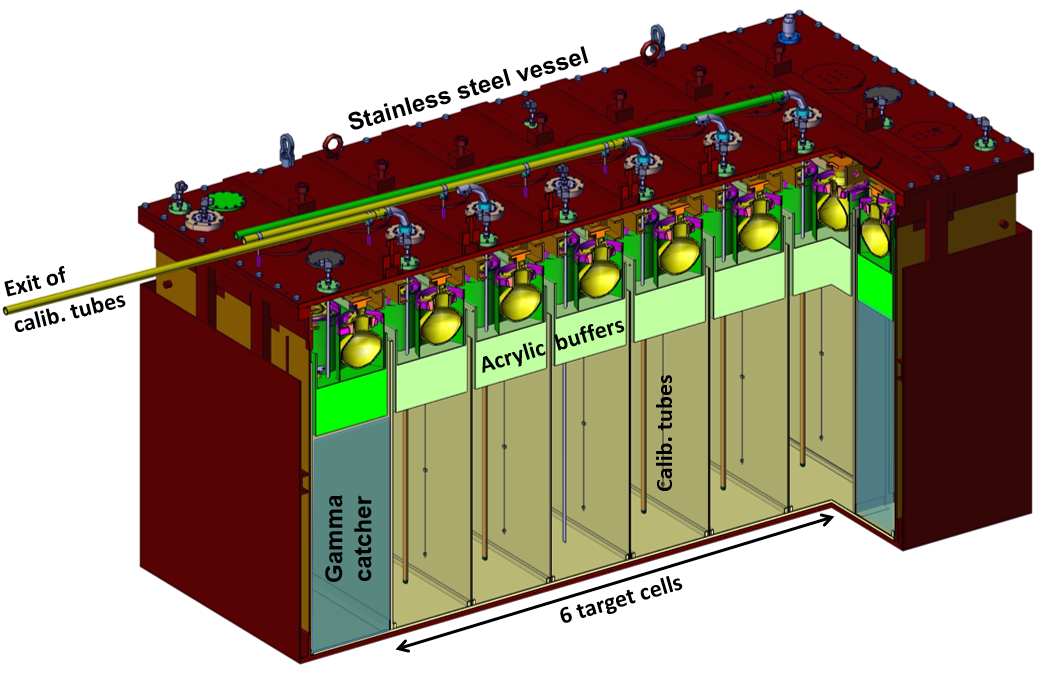
\includegraphics[width=0.8\linewidth]{images/Detector_3D_CutView.png} 
\caption[Coupe schématique du détecteur]{Coupe schématique du détecteur laissant apparaitre les cellules de la Target ainsi que celles du Gamma-Catcher. (source : \cite{docdb225})} 
\label{fig:Detector_3D_CutView.png} 
\end{figure} 

} 

Chaque paroi en acrylique est constituée de deux plaques fines collées sur leur pourtour et contenant une couche réfléchissante qui permet d'assurer la séparation optique cellule à cellule ainsi que limiter les effets de volume sur la collection de lumière. Le matériau utilisé est l'ESR (Enhanced Specular Reflector) produit par 3M. Le fournisseur garantit une réflexivité supérieure à 99 \% pour des longueurs d'onde du spectre visible, lorsque le matériau est plongé dans l'air (voire Figure \ref{fig:cell_reflectivity.jpg}). Cependant, plongé dans le liquide, ou en contact optique avec l'acrylique, ce dernier perd en réflectivité lorsque l'angle d'incidence des photons est trop grand ($> 60^{\circ}$). Un fin voile de nylon de $\SI{100}{\mu m}$ d'épaisseur est donc inséré à l'intérieur de chaque "sandwich" acrylique. Il assure la présence d'un gap d'air à l'interface avec l'ESR qui permet de garder ses propriétés réfléchissantes originales.\\ 

\afterpage{ 

\begin{figure}[h!] 
\centering 
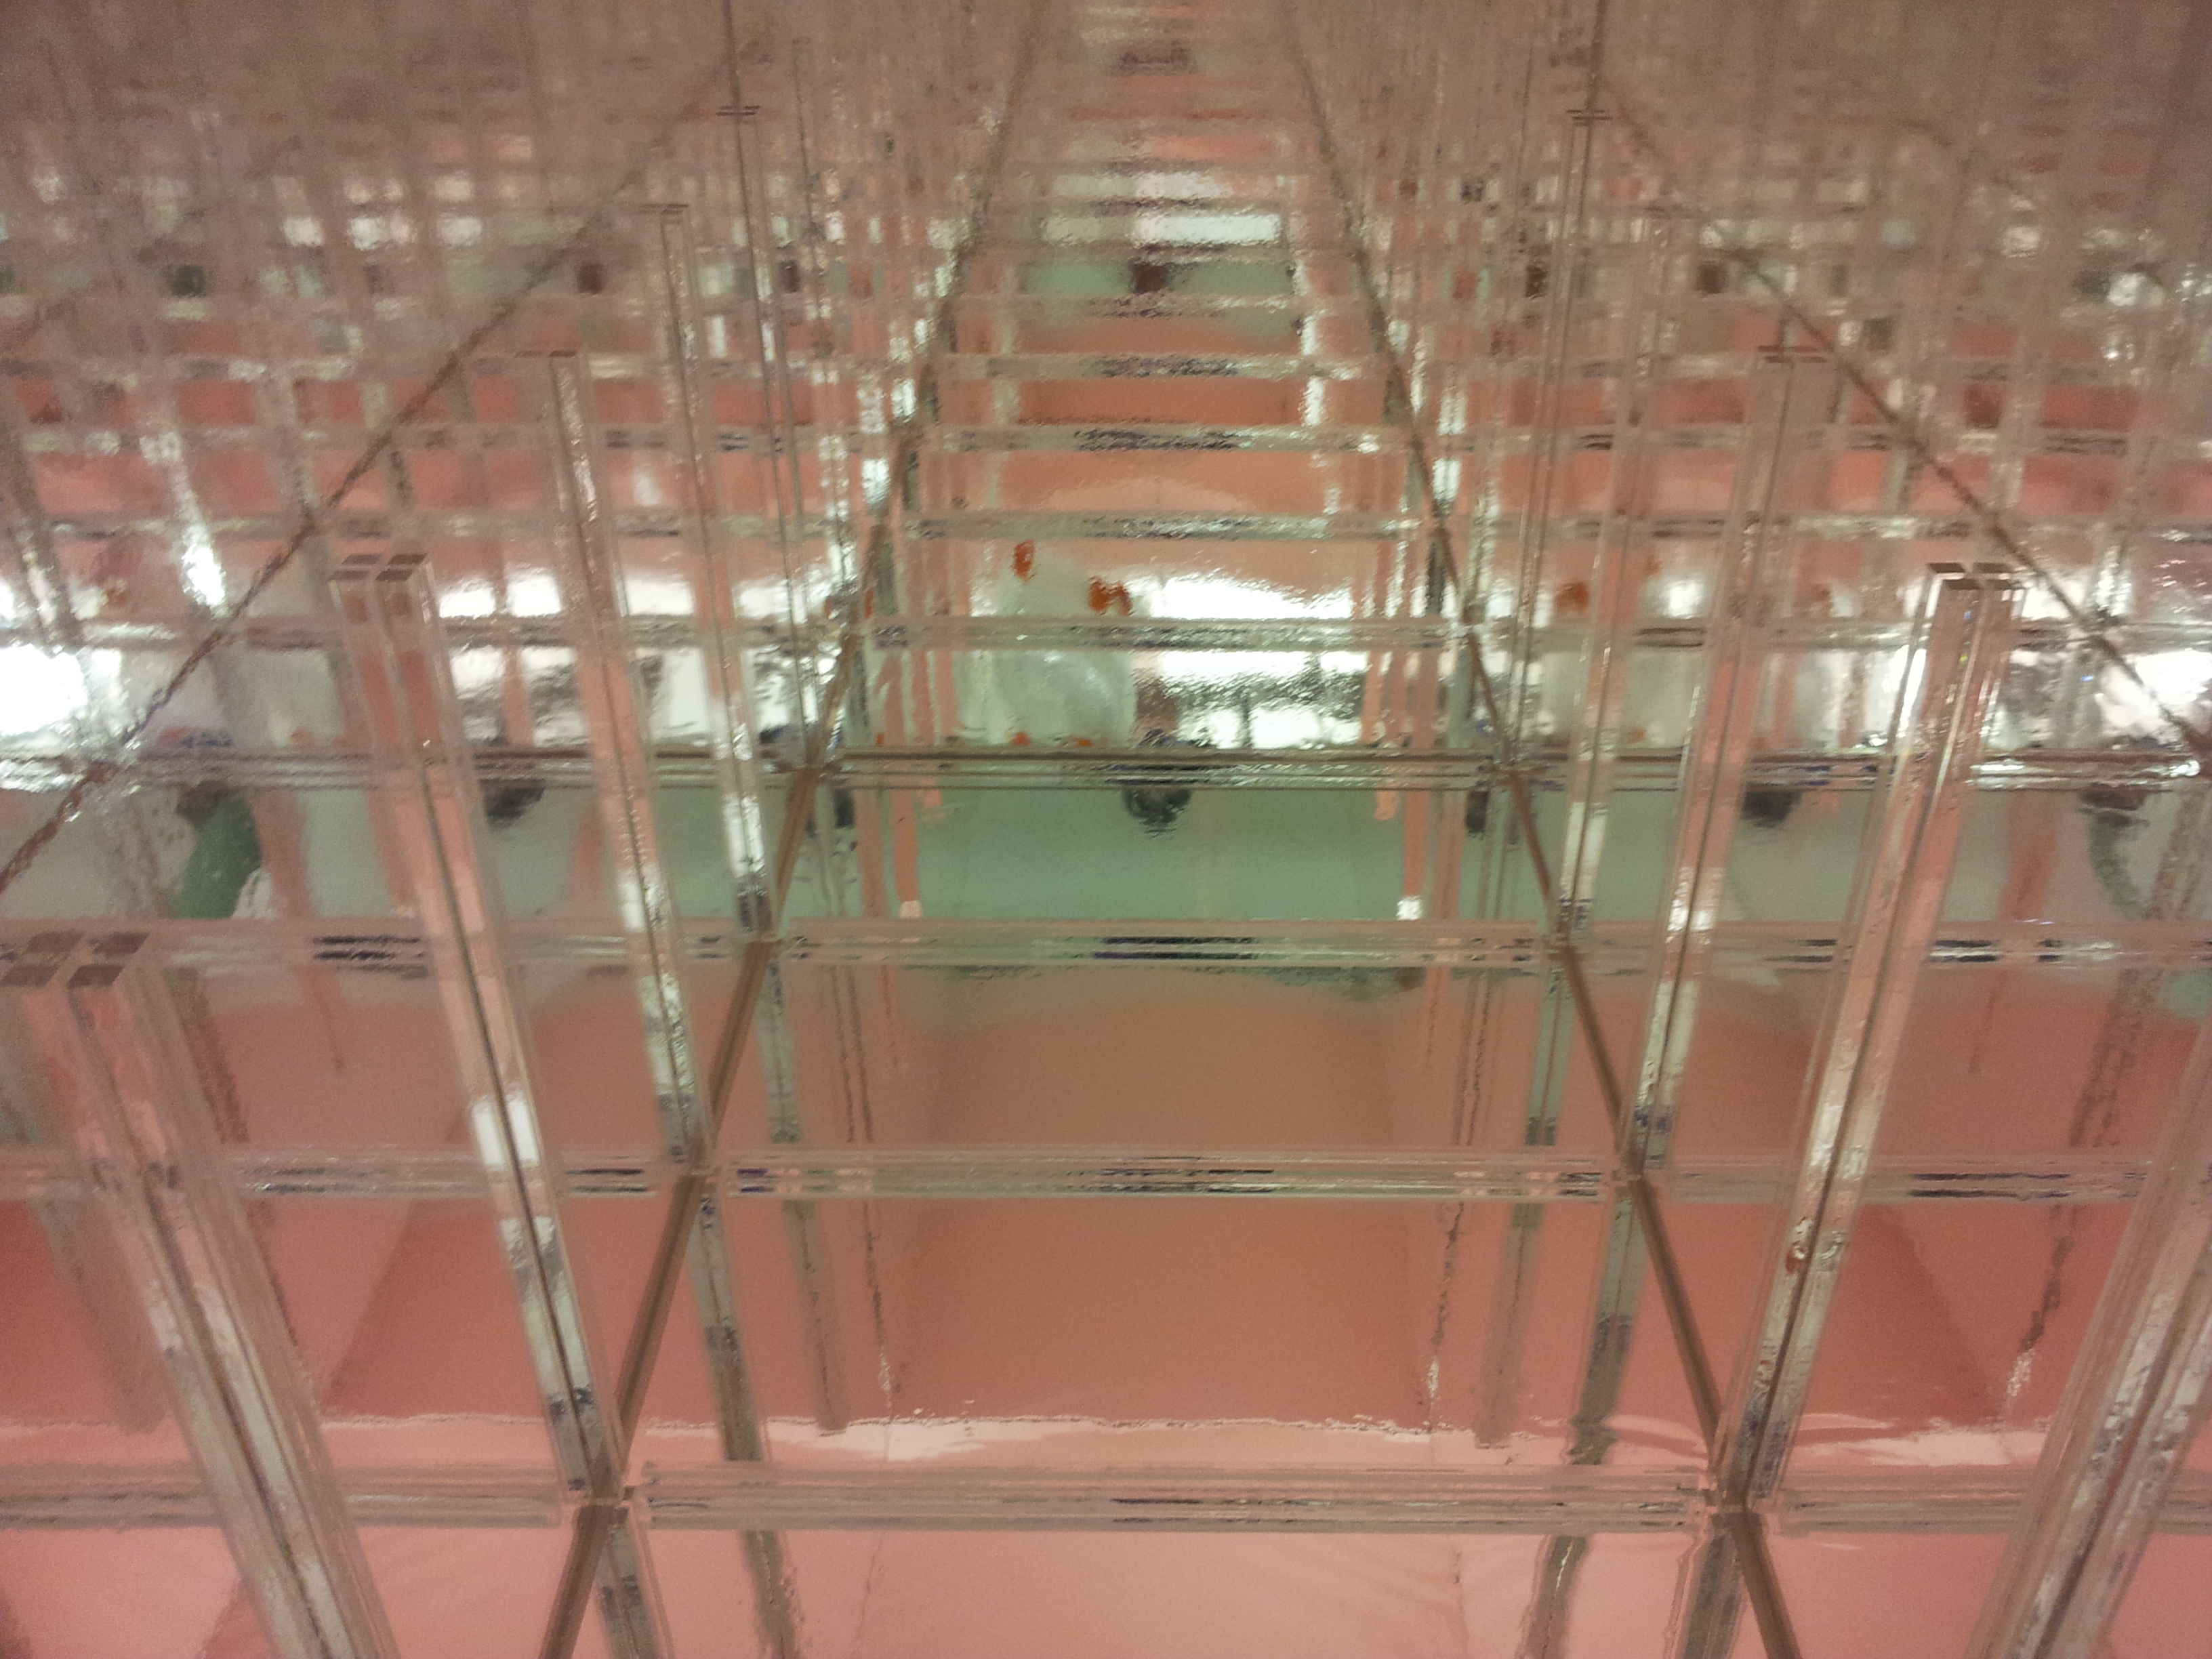
\includegraphics[width=0.9\linewidth]{images/cell_reflectivity.jpg} 
\caption[Photos d'une cellule de \textsc{Stereo} avec ses parois réfléchissantes]{Photos d'une cellule de \textsc{Stereo} avec ses parois réfléchissantes.} 
\label{fig:cell_reflectivity.jpg} 
\end{figure} 

} 

\bigbreak 

\subsection{Propriétés du liquide scintillateur} 

Le liquide est constitué principalement de LAB (Linear Alkyl Benzene) à $\sim 75 \%$, de PXE (ortho-phenylxylylethane) à $\sim 20 \%$ et de DIN (diisopropylnaphtalene) à $\sim 5 \%$ \cite{Buck:2018cac}. Le choix de ces produits est conduit par les spécifications de $\textsc{Stereo}$ à savoir : bonne transparence, haut rendement lumineux, Pulse Shape Discrimination (PSD) et radiopureté. Le liquide doit aussi satisfaire les contraintes de sureté inhérentes au site de l'ILL comme la température du point d'éclair, ou encore ne pas entrainer de réaction chimique avec les autres matériaux du détecteur. Le solvant principal qui a été choisi est le LAB, car relativement inerte chimiquement, mais ce dernier n'atteint pas les spécifications sur la discrimination des neutrons rapides. Pour cela, du PXE et du DIN ont été ajoutés au (léger) détriment de la transparence. Le gadolinium est mis en suspension grâce à une molécule organique l'encapsulant ($\ce{Gd(thd)_3}$) qui assure une grande stabilité de la dissolution du Gd et minimise ses effets sur la transparence du liquide. Du reste, d'autres molécules sont utilisées, comme le tetrahydrofuran pour minimiser les risques d'inflammation ou encore du diphenyloxazole et du bis-methylstyrylbenzene pour décaler la longueur d'onde des photons de scintillation et maximiser l'efficacité de collection des photomultiplicateurs. La composition du liquide est résumée dans le Tableau \ref{tab:liquid_composition}.\\ 

\afterpage{ 

\centering 
\begin{table}[h!] 
\begin{tabular}{|c|c|c|c|c|} 
\hline 
Composante & Fonction principale & Fraction de masse & Masse molaire & $N_H$ \\ 
\hline 
\hline 
\multirow{2}{*}{LAB} & Rendement lumineux & \multirow{2}{*}{73 \%} & \multirow{2}{*}{246 g/mol} & \multirow{2}{*}{30}\\ 
& + protons cibles & & & \\
\hline 
\multirow{2}{*}{PXE} & Rendement lumineux & \multirow{2}{*}{19,5 \%} & \multirow{2}{*}{210 g/mol} & \multirow{2}{*}{18}\\ 
& + Discrimination neutrons & & & \\
\hline 
DIN & Discrimination neutrons & 4,9 \% & 212 g/mol & 20\\ 
\hline 
$\textrm{Gd}(\textrm{thd})_3$ & Capture neutrons & 2,2 & 707 g/mol & 57\\ 
\hline 
tetrahydrofuran (THF) & Sûreté & 0,9 \% & 72 g/mol & 8\\ 
\hline 
PPO & Wavelength Shifter & 0,8 \% & 221 g/mol & 11\\ 
\hline 
Bis-MSB & Wavelength Shifter & 0,002 \% & 310 g/mol & 22\\ 
\hline 
\end{tabular} 
\caption[Composition du liquide scintillateur]{Composition du liquide scintillateur. $N_H$ est le nombre de proton que possède chaque molécule.} 
\label{tab:liquid_composition} 
\end{table} 

} 

Le liquide obtenu a un rendement lumineux d'environ 7000 photons par MeV et les photons sont principalement émis entre 375 et $\SI{450}{nm}$, bande passante où l'efficacité quantique des PMs est maximale. La longueur d'atténuation qui a été mesurée en laboratoire est en accord avec la prédiction\footnote{La valeur théorique est obtenue avec : $\frac{1}{\Lambda} = \frac{1}{\Lambda_{LAB}} + \frac{1}{\Lambda_{PXE}} + \frac{1}{\Lambda_{DIN}}...$. Un écart significatif avec la valeur mesurée aurait signifié un problème de propreté du détecteur ou de pureté des composants chimiques employés.} : $\SI{6.9}{m}$. Cette valeur est satisfaisante, car elle reste très grande devant les dimensions caractéristiques des cellules. Enfin, pour conserver ces propriétés de scintillation dans le temps, une atmosphère d'azote en légère surpression (20 millibars) est constamment maintenue au-dessus du liquide pour limiter l'absorption de l'oxygène par le liquide.\\ 

Puisque chacune des composantes décrites dans la Table \ref{tab:liquid_composition} sont des molécules organiques, l'essentiel des protons cibles pour héberger les réactions IBD se trouvent dans le liquide scintillateur. Le contrôle du nombre de protons est crucial pour estimer le taux d'interactions des neutrinos dans le détecteur, car son incertitude associée se répercute directement sur la mesure du flux d'antineutrinos détectés. De plus, le rapport entre le nombre de noyaux d'Hydrogène et de gadolinium affecte le spectre de captures des neutrons et donc l'efficacité de détection. Le nombre de protons peut être obtenu de la masse du liquide : 

\begin{equation} 
N_p = \frac{f_H M_L}{m_p},
\end{equation} 

\bigbreak 

où $f_H$ est la fraction de masse Hydrogène du liquide, $M_L$ la masse du liquide et $m_p$ la masse du proton. $f_H$ a été mesuré à l'Université technique de Munich (TUM) par \og \textit{elemental analysis} \fg{} avec une précision relative de l'ordre du \% : $f_H = \left( 11,45 \pm 0,11 \right) \%$ \cite{docdb517}. La masse du liquide quant à elle a été mesurée lors du remplissage du détecteur: $M_L = (1602 \pm 2) \SI{}{kg}$.\\ 

%\begin{itemize} 
% \item Composition du liquide / 
% \item Longueur d'onde / Longueur d'atténuation 
% \item Dopage et encapsulation Gd 
% \item Mesures de conservation du liquide (injection permanente azote) 
%\end{itemize} 

\subsection{Conversion de la lumière par les photomultiplicateurs} 

Les photomultiplicateurs possèdent une photocathode de 8 pouces de diamètre (R5912-100) qui permet de maximiser la surface de collection globale de chaque cellule. L'efficacité quantique de chaque PM est de 30 \% en moyenne sur le spectre d'émission du liquide. Un photon interagissant avec la photocathode génère un électron qui est déporté vers une chambre d'amplification. Une cascade d'électrons est déclenchée et charge un condensateur au niveau de l'anode. Ce dernier se décharge avec une constante de temps propre au circuit RC qui est implémenté. L'évolution de la tension aux bornes de ce circuit est enregistrée par un système d'acquisition à l'extérieur du détecteur. En pratique plusieurs photons sont collectés sur la photocathode et génèrent plusieurs avalanches électroniques. La charge collectée par le condensateur est directement proportionnelle au nombre de photons captés par la photocathode. Le nombre de photons incidents est donc mesuré en comparant l'intégrale de la tension en sortie du PM avec une valeur de référence: 

\begin{equation} 
Q_{tot} = \frac{\int_{0}^{T} V(t) dt}{K}, 
\label{eq:Qtot_def}
\end{equation} 

\bigbreak 

où l'intervalle $[0,T]$ représente la fenêtre temporelle encapsulant le pulse (charge + décharge du condensateur), $V$ la tension en fonction du temps et $K$ une constante d'étalonnage.\\ 

% La constante $K$ est obtenu en injectant une infime quantité de lumière dans le détecteur par des fibre optique conduisant la lumière produite par des LEDs.\\ 

\bigbreak 

%\begin{itemize} 
% \item Disposition des PMTs dans le détecteur 
% \item Exemple forme impulsion 
% \item Conversion en PE 
%\end{itemize} 

\subsection{Système d'acquisition des données} 
\label{sec:stereo_elec} 

Un système électronique d'acquisition a été développé spécialement pour l'expérience \textsc{Stereo}. Il sert plusieurs rôles: système de déclenchement de l'acquisition (triggering), conversion signaux analogiques vers numériques (ADC), traitement du signal, système de consultation (readout), et système de calibration en ligne (on-line calibration) \cite{Bourrion:2015axa}.\\ 

Les 68 voies de sortie des PMs (48 détecteurs + 20 vetos) sont recueillies par des cartes \textit{Front End} (FE) où les tensions sont numérisées avec un taux d'échantillonnage à $\SI{250}{MHz}$, soit un échantillon toutes les $\SI{4}{ns}$. Les données numérisées sont traitées en ligne par un filtre à réponse impulsionnelle infinie (filtre passe-haut au premier ordre) qui corrige la ligne de base et envoie les données en parallèle dans un module de \textit{triggering} ainsi que dans une mémoire tampon circulaire (\textit{buffer}). Le déclenchement de l'acquisition est effectué par des conditions sur l'amplitude ou la charge des signaux, sommées sur plusieurs voies de PMs (T1). En parallèle, plusieurs variables sont calculées à partir des données stockées dans le \textit{buffer} circulaire: $t_{CFD}$, $Q_{tot}$ et $Q_{tail}$. Le temps défini par discrimination à fraction constante ($t_{CFD}$) permet de fixer le zéro marquant le début du pulse. La charge totale $Q_{tot}$ est calculée sur le principe de l'Équation (\ref{eq:Qtot_def}) en intégrant à partir de quelques microsecondes avant $t_{CFD}$ (pour ne pas manquer la montée du signal). La variable $Q_{tail}$ quant à elle est obtenue en déplaçant le début de la porte d'intégration de $\SI{65}{ns}$ \cite{docdb409} afin de ne considérer la charge que dans la queue du pulse. C'est cette variable qui permet d'évaluer l'amplitude de la composante retardée du processus de scintillation (cf. section \ref{seq:scintillation}). Ces trois variables sont représentées sur la figure \ref{fig:PSD_real.pdf}.\\ 

Si les critères de sélection sont satisfaits, les données traitées de chaque voie sont agrégées pour être analysées par un autre module effectuant des sélections de second niveau (T2). Des conditions sur la charge totale recueillie par tous les PMs du détecteur, de même que celle recueillie par le véto muon, permettent de s'affranchir de certains bruits de fond à la volée \cite{docdb179}. Si les conditions de (T2) sont respectées, les observables sont écrites sur disque dur. Il est important de noter que seules les observables d'intérêt sont conservées en fin de chaine. En effet, l'enregistrement complet de la forme des pulses peut être effectué, mais au prix d'un temps mort considérable rendant la recherche de paires positron-neutron impossible. Ce mode d'acquisition (mode \textit{debug}) a en revanche servi à optimiser la porte d'intégration de $Q_{tail}$ afin de maximiser l'efficacité de la PSD. En mode normal, le taux d'acquisition maximal est de $\SI{3.6}{MHz}$ (soit un événement toutes les $\SI{0.3}{\mu s}$ en négligeant le temps mort).\\ 

L'amplitude du bruit électronique est un ordre de grandeur inférieure au photo-électron. Cela permet de mesurer la quantité de photons collectés dans le détecteur avec une incertitude inférieure à $\pm \SI{1}{}$ p.e.. De même, la linéarité de la réponse a été testée en utilisant un réseau de LEDs qui injecte de la lumière directement sur les PMs via des fibres optiques. En comparant la charge mesurée avec des photons émis par une combinaison de diodes d'intensités différentes et la charge mesurée par diode individuelle, la linéarité a été contrainte sur toute la gamme du spectre neutrino (voire figure \ref{fig:Linearity_Target.pdf}): $< 1 \%$ jusque $\SI{10}{MeV}$.\\ 

\afterpage{ 

\begin{figure}[h!] 
\centering 
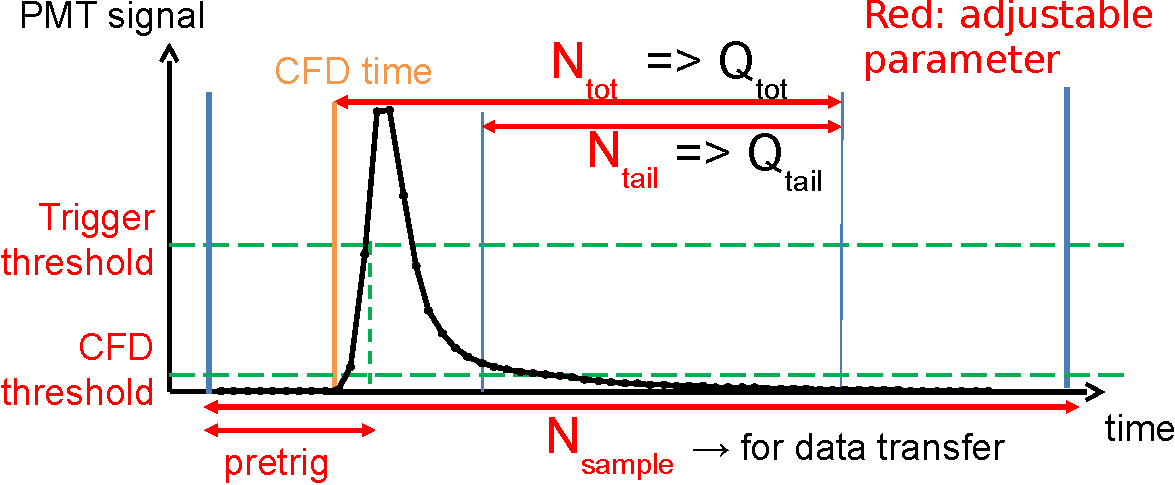
\includegraphics[width=0.8\linewidth]{images/PSD_real.pdf} 
\caption[Représentation d'une impulsion en sortie d'un photomultiplicateur]{Représentation d'une impulsion en sortie d'un photomultiplicateur numérisée d'où sont extraites les observables d'intérêt : $t_{CFD}$, $Q_{tot}$ et $Q_{tail}$. (source : \cite{salagnac:tel-01757168})} 
\label{fig:PSD_real.pdf} 
\end{figure} 

\begin{figure}[h!] 
\centering 
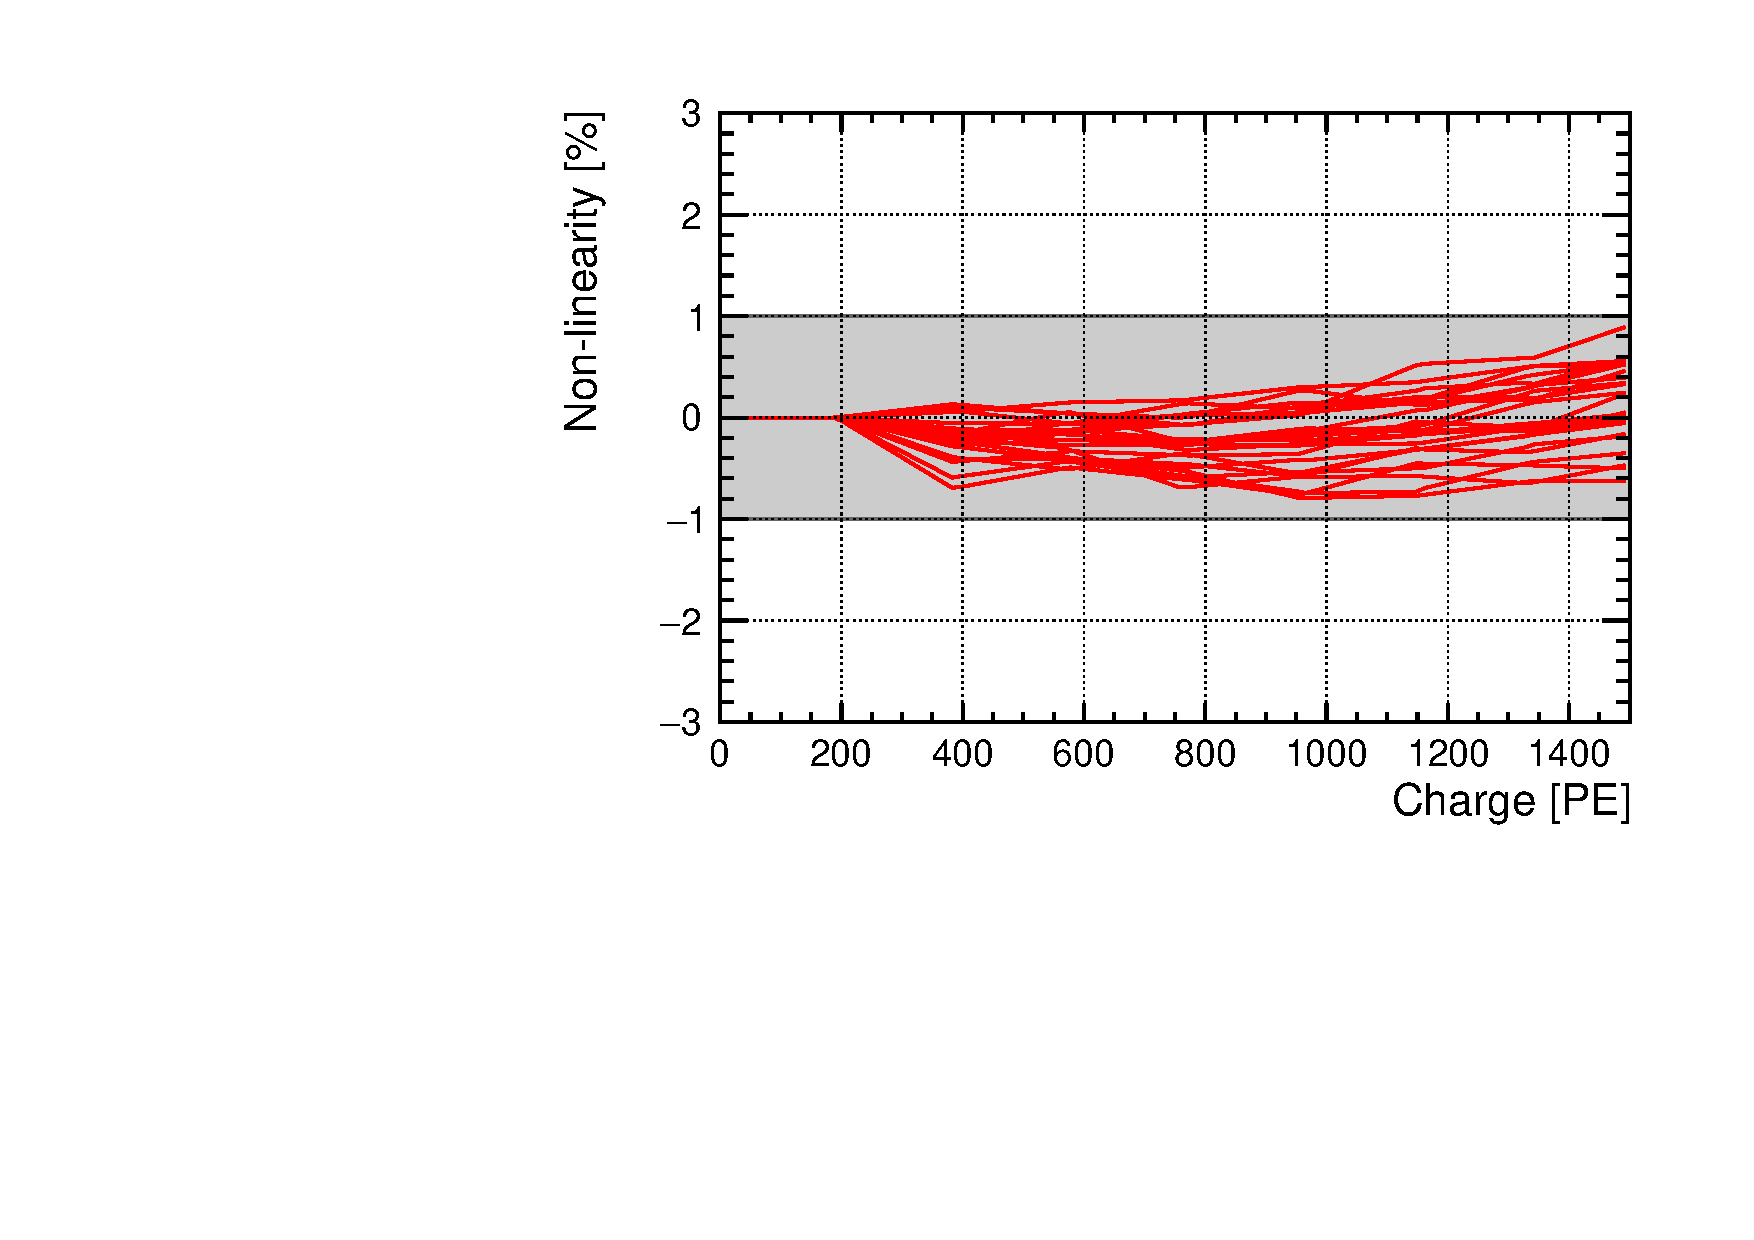
\includegraphics[width=0.8\linewidth]{images/Linearity_Target.pdf} 
\caption[Écarts typiques à la linéarité de la chaîne d'acquisition de \textsc{Stereo}]{Écarts typiques à la linéarité de la chaîne d'acquisition de \textsc{Stereo}, mesurés en réponse à des combinaisons linéaires de pulses lumineux envoyés sur les PMs. La gamme testée correspond à des énergies déposées dans la cellule jusqu'à plus de 10 MeV. (source \cite{Allemandou:2018vwb})} 
\label{fig:Linearity_Target.pdf} 
\end{figure} 

\begin{figure}[h!] 
\centering 
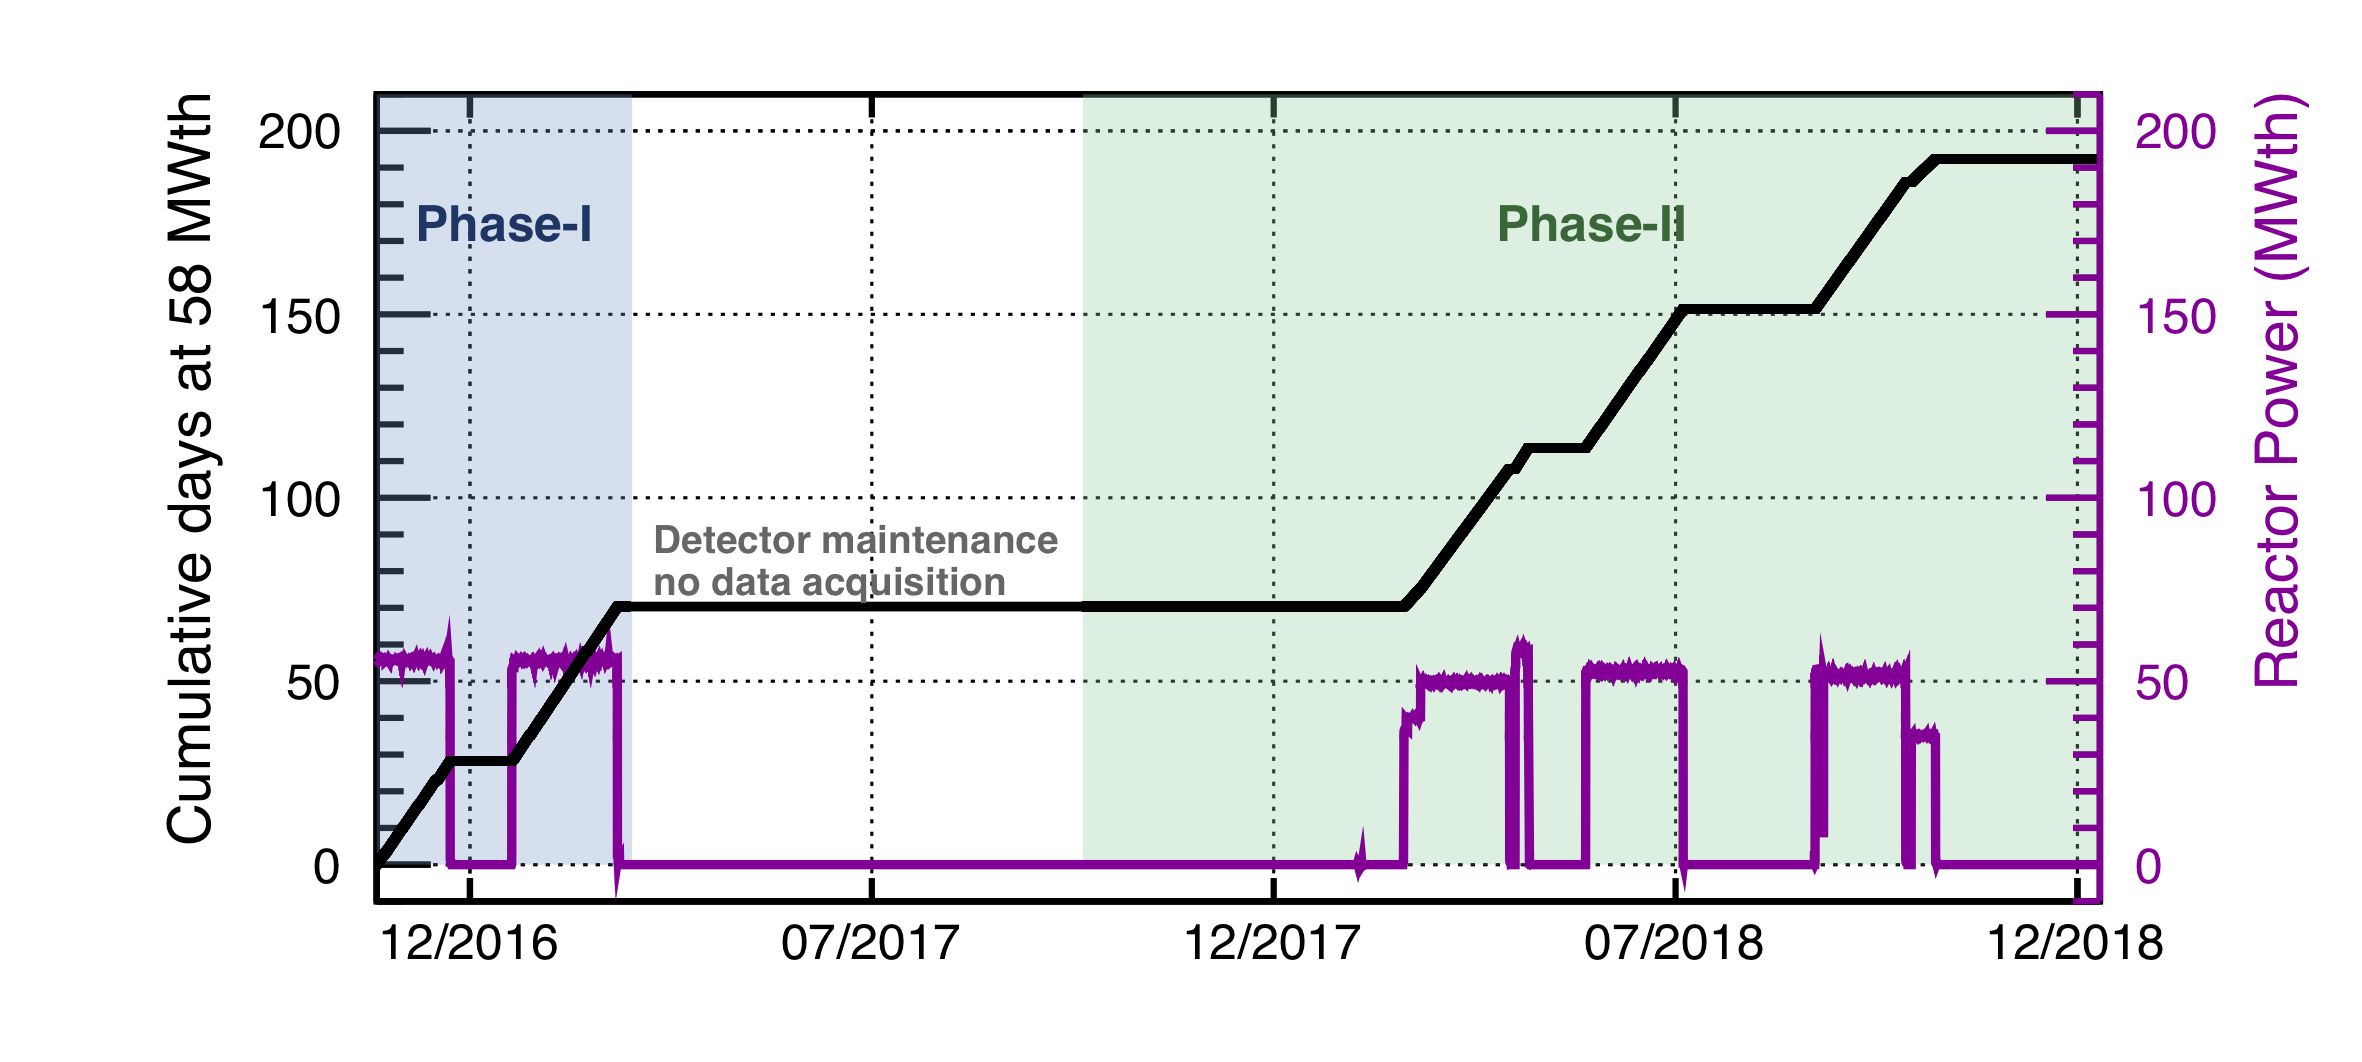
\includegraphics[width=0.8\linewidth]{images/DataTaking_phase12.png} 
\caption[Résumé de la prise de donnée \textsc{Stereo} entre fin 2016 et fin 2018]{Résumé de la prise de donnée \textsc{Stereo} entre fin 2016 et fin 2018. (source : \cite{docdb886})} 
\label{fig:DataTaking_phase12} 
\end{figure} 

\clearpage 

} 

\bigbreak 

% 
%\begin{itemize} 
% \item ADC -> Quelles observables energistrés 
% \item temp mort 
% \item Non linéarités ? 
%\end{itemize} 

\subsection{Stockage des données et prétraitement} 

La prise de donnée est interfacée par un programme basé sur NOMAD, un logiciel de contrôle d'acquisition centralisé qui est développé par l'ILL \cite{docdb83}. Ce programme permet notamment de suivre diverses grandeurs sur l'environnement de \textsc{Stereo} comme: les hautes tensions des PMs, la température du liquide ou de l'électronique, le niveau du liquide scintillateur, ou encore la pression. Une des fonctions principales du programme est de contrôler l'acquisition des données sur disque dur. Des macros qui résument l'ensemble des paramètres (durée d'acquisition, triggers, gain ADC, LEDs...) propres à un mode de prise de données sont stockées et prêtes à l'emploi. Par exemple, la personne en charge de la prise de données peut interrompre l'acquisition "type neutrino", puis changer les \textit{presets} pour effectuer une calibration avec les paramètres de déclenchement adéquats. Chaque période de prise de données continue avec un même jeu de paramètres de déclenchement est appelée \og \textit{run} \fg{} et est estampillée d'une chaine de caractère représentant la date à laquelle le programme a commencé à prendre des données; par exemple un run qui commence le $1^\textrm{er}$ janvier 2019 à 12h 00min 00s, sera étiqueté : 20190101\_120000.\\ 

Les données acquises avec les paramètres de déclenchement relatifs aux signaux neutrinos sont découpées en runs d'une heure pour éviter de perdre une trop grande quantité de données si l'acquisition vient à s'arrêter spontanément. Une fois terminés, les runs au format \og \textit{Raw} \fg{} sont transférés sur un espace de stockage au LPSC de Grenoble et les paramètres d'acquisition sont écrits sur une base de données mySQL.\\ 

Un centre de calcul au LPSC est sollicité pour effectuer la phase de \og \textit{Preprocessing} \fg{}. Cette dernière consiste à convertir les données binaires (\textit{Raw}) en fichiers dits \og \textit{Preprocessed} \fg{} lisibles par les utilisateurs à l'aide de ROOT, la bibliotèque développée par le CERN. Chaque fichier ROOT rassemble les paramètres d'acquisition, le temps du run, la position des PMs, et un arbre \og \textit{Data} \fg{} dans lequel sont stockées la charge en photo-électron des PMs et la date de déclenchement pour chaque signal enregistré. Une fois la phase \textit{Preprocessing} terminée, les fichiers ROOT sont transférés sur bandes magnétiques à Lyon, dans l'espace de stockage attitré \og HPSS \fg{}. Dès lors, les données sont accessibles à la collaboration \textsc{Stereo} depuis le centre de calcul de Lyon.\\ 

Par ailleurs, puisque l'emplacement de \textsc{Stereo} hérite de contraintes inhérentes à une zone reglementée à propos de la sûreté nucléaire, un dispositif de surveillance par la \textit{control room} du réacteur a été mis en place pour mesurer et alerter si besoin des anomalies concernant la température, le niveau des liquides ou encore la pression dans l'enceinte.\\

% TODO FM : Comment sont rendus dispo ces données de surveillance / databas ? fichier dédié ?

\bigbreak 

\section{Prise de données} 

Le détecteur \textsc{Stereo} a commencé à prendre des données devant le réacteur de l'ILL à partir du 11 novembre 2016. La première période de fonctionnement du détecteur s'est déroulée jusqu'au 12 mars 2017. Cette première phase de prise de données a permis d'accumuler 84 jours de données avec un réacteur à pleine puissance, mais aussi 32 jours de périodes d'arrêts. La prise de données a été interrompue par une longue période d'arrêt du réacteur dédiée à divers travaux de maintenance. En particulier, la nécessité de changer la gaine du tube faisceau H7 a contraint \textsc{Stereo} de se retirer de la casemate pendant quelques mois. La seconde phase de prise de donnée a débuté le 29 septembre 2017. \textsc{Stereo} a mesuré le bruit de fond cosmique pendant une centaine de 100 jours avant que l'ILL ne reprenne les cycles de fonctionnement habituels au 1$^\textrm{er}$ mars 2018. Le réacteur s'est de nouveau arrêté le 29 octobre 2018 pour laisser place à une longue période de shutdown. Pour résumer, la prise de données \textsc{Stereo} est représentée par la figure \ref{fig:DataTaking_phase12}.\\ 

\subsection{Assemblage et mise en marche} 
\label{sec:assemblage} 

\bigbreak 

Le détecteur interne a été assemblé en mars-avril 2016 dans le hall Ariane du LPSC à Grenoble. La figure \ref{fig:team_bbr.png} montre une photo du détecteur interne une fois assemblé dernière les scientifiques de \textsc{Stereo} qui ne cachent pas leur enthousiasme! En mai 2016, le détecteur ainsi que les blindages ont été acheminés sur le site de l'ILL (voire figure \ref{fig:stereo_trans.png}). Les blindages internes et externes ont finalement été installés pendant l'été 2016, et le remplissage du liquide scintillateur a été effectué le 10 novembre 2016, une fois le feu vert annoncé par l'ASN (Autorité de Sûreté Nucléaire).\\ 

\afterpage{ 

\begin{figure}[h!] 
\centering 

\begin{subfigure}[b]{0.49\textwidth} 
\centering 
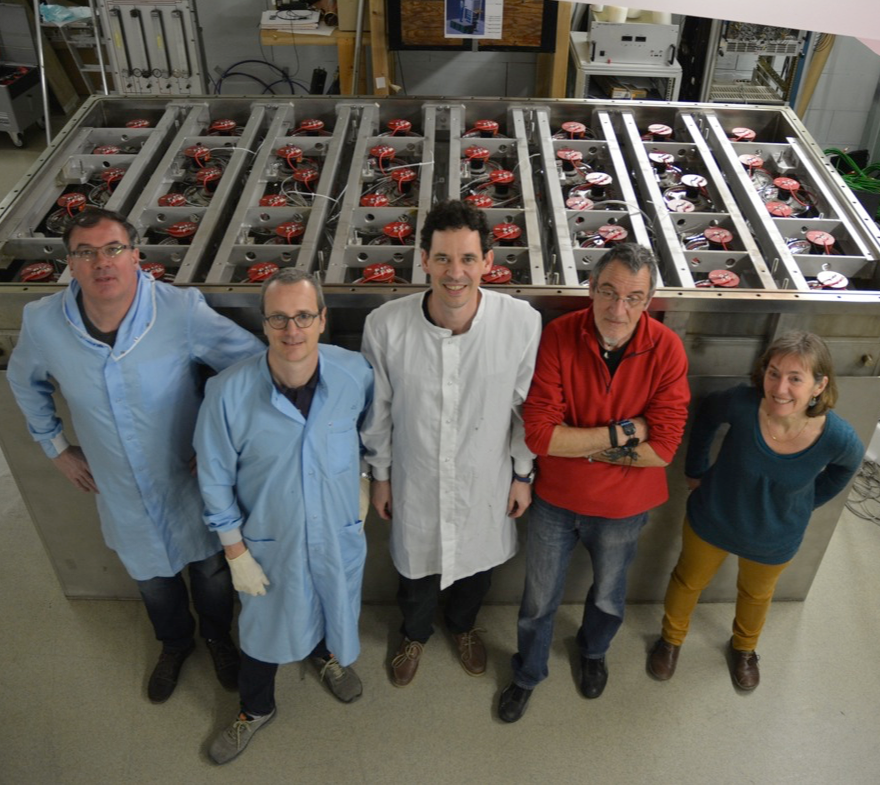
\includegraphics[width=1\linewidth]{images/team_bbr.png} 
\caption{Le détecteur interne après l'assemblage derrière l'équipe \og bleu-blanc-rouge \fg{}. De gauche à droite : Gilles COULLOUX, Loris SCOLA, David LHUILLIER, Patrick CHAMPION, Anne STUTZ.} 
\label{fig:team_bbr.png} 
\end{subfigure} 
~ % attention ! space sensitive 
\begin{subfigure}[b]{0.49\textwidth} 
\centering 
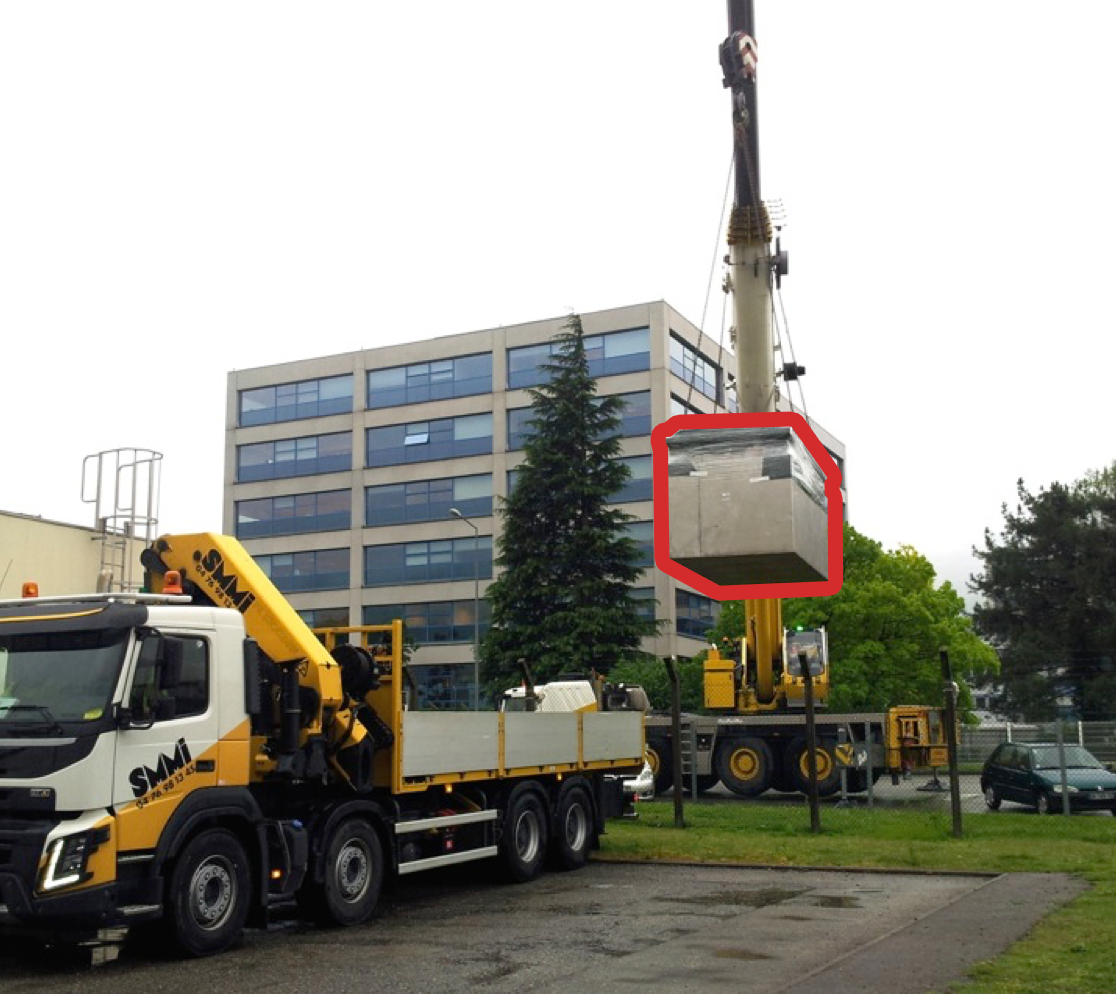
\includegraphics[width=1\linewidth]{images/stereo_trans.png} 
\caption{Grue mobile transportant le détecteur interne (entouré en rouge) du site LPSC au site ILL.} 
\label{fig:stereo_trans.png} 
\end{subfigure} 
\caption[Photos de l'assemblage et du transport de \textsc{Stereo} à l'ILL]{Photos de l'assemblage et du transport de \textsc{Stereo} à l'ILL.} 
\label{fig:} 
\end{figure} 

} 

Durant les deux semaines suivant la mise en service, de nombreux paramètres instrumentaux ont été ajustés afin d'assurer la qualité des données. Finalement, le taux de déclenchement de l'acquisition est de $\SI{1}{kHz}$ pour un seuil équivalent à $\sim \SI{300}{keV}$ avec temps mort inférieur à $\SI{0.2}{\%}$. Une étude préliminaire a été menée pour identifier les bruits de fonds dominants dans le cadre de cette thèse. Le taux de comptage dans la fenêtre en énergie Prompt est de l'ordre de $\SI{15}{Hz}$ et lorsque l'expérience IN20 est en marche, ce taux augmente jusqu'à $\SI{20}{\%}$. La composante de bruit de fond la plus importante à basse énergie provenait de la décroissance des noyaux d'$\ce{^{41}Ar}$. En effet, les neutrons qui interagissent avec l'air dans le hall expérimental entrainent la production de noyaux d'$\ce{^{41}Ar}$ ayant une durée de vie d'environ 2 heures. L'$\ce{^{41}Ar}$ se désintègre par décroissance beta, et son noyau fils ($\ce{^{41}K}$) se désexcite en émettant un gamma d'environ $\SI{1.3}{MeV}$. Le renouvellement de l'air dans les tubes de calibration entrainait la propagation de gammas dans le liquide scintillateur. Des bouchons en plomb et polyéthylène ont été placés en sortie des tubes de calibration afin de limiter le renouvellement de l'air et la propagation de bruits de fond par ces entrées.\\ 

Des défaillances techniques se sont rapidement manifestées. Tout d'abord, deux buffers en acrylique ont subi des dommages probablement causés lors des déplacements de \textsc{Stereo}. L'huile au-dessus des buffers des cellules 4 et 0 (cellule du Gamma-Catcher juste devant la cellule 1) a fui et lesdites cellules ont perdu le couplage optique avec leurs photomultiplicateurs: la collection de lumière a chuté de $\SI{60}{\%}$ dans ces cellules. De plus, l'augmentation significative des fuites de lumière d'une cellule à une autre a témoigné d'une certaine perte de réflectivité de la majorité des plaques séparant chaque cellule, et a ainsi complexifié la correspondance entre charge détectée et énergie déposée. L'évolution des fuites de lumière est exposée sur la figure \ref{fig:LL_phase_1}. L'origine du problème a été identifiée comme la perte d'étanchéité du joint de colle à la périphérie des plaques acryliques, permettant l'entrée de liquide scintillant dans le gap d'air interne. La phase de maintenance de l'été 2017 a permis d'entreprendre des réparations avant la seconde phase de prise de données. Les fuites lumière sont désormais stables depuis presque deux ans (voire figure \ref{fig:LL_phase_2}) et les fuites entre cellules cibles ont été réduites.\\ 

\afterpage{ 

\begin{figure}[h!] 
\begin{subfigure}[b]{0.5\textwidth} 
\centering 
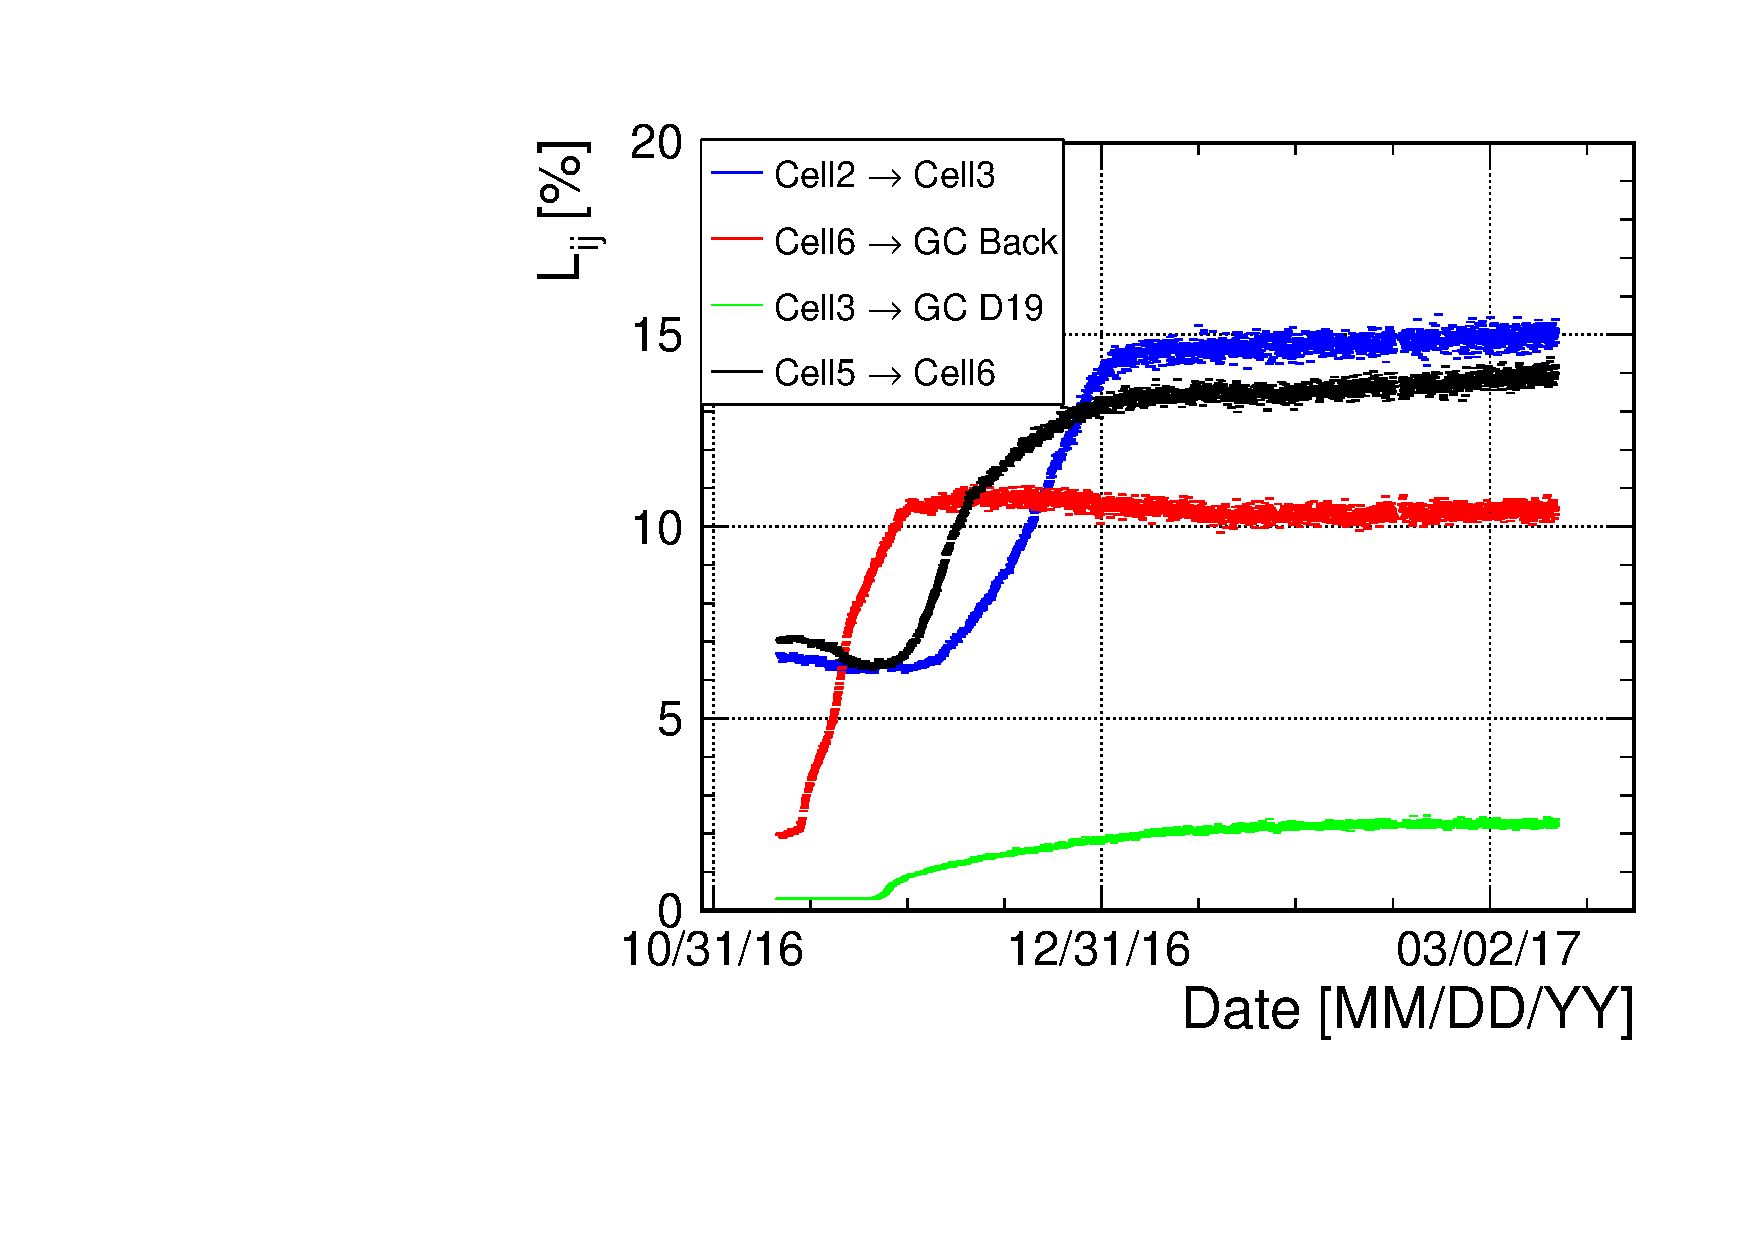
\includegraphics[width=1\linewidth]{images/LLEvolution1.pdf} 
\caption{} 
\label{fig:LL_phase_1} 
\end{subfigure} 
~ % attention ! space sensitive 
\begin{subfigure}[b]{0.5\textwidth} 
\centering 
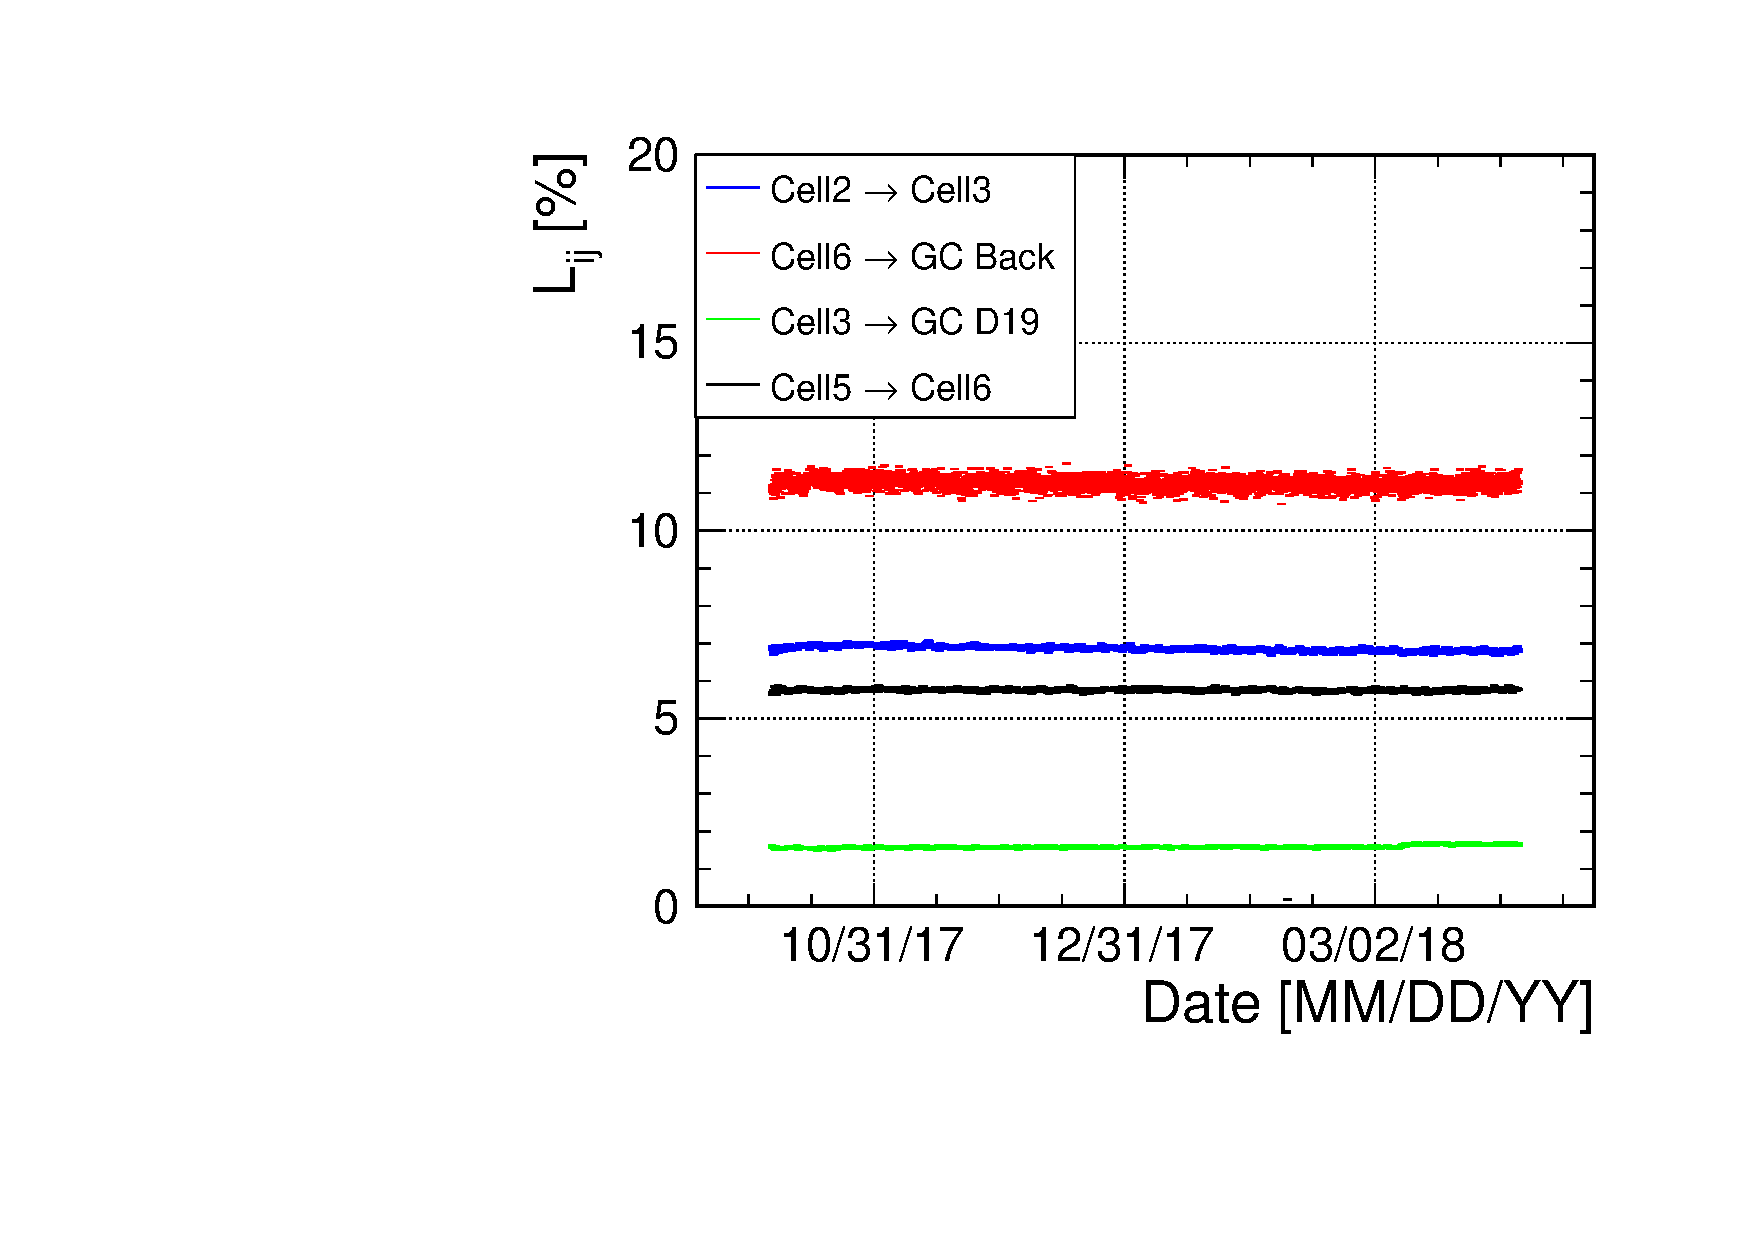
\includegraphics[width=1\linewidth]{images/LLEvolution2.pdf} 
\caption{} 
\label{fig:LL_phase_2} 
\end{subfigure} 
\caption[Évolution des fuites de lumière pendant la Phase-I et la Phase-II]{Évolution des fuites de lumière pendant la Phase-I (a) et la Phase-II (b). Ces coefficients sont mesurés via les muons cosmogéniques. La méthode est détaillée dans la section \ref{sec:LL_JS}. (source \cite{Allemandou:2018vwb})} 
\label{fig:LL_phase_1_2} 
\end{figure} 

} 

\bigbreak 

%\begin{itemize} 
% \item Commissioning 
% \item Trigger rates 
%\end{itemize} 
%\subsection{Examen et réparations après la première phase} 
%\label{sec:detector_repair} 
% 
%La période de retrait de \textsc{Stereo} entre les deux phases de prise de données a été mise à profit de l'examen et des réparations du détecteur interne. Les fuites d'huile assurant le contact optique ont été causées par des fissures dans les buffers en acrylique au niveau de joints où des pièces d'acrylique sont emboitées ou collées. Le \textit{buffer} du bloc frontal du Gamma Catcher a subi des dommages au niveau d'un bord de l'aquarium, alors que celui de la cellule 4 a fui à cause de l'ouverture d'une fissure au niveau de l'emplacement où passe le tube de calibration en inox. Ces défaillances ont probablement été causées par des contraintes trop intenses appliquées lors de l'acheminement du détecteur à la casemate. La figure \ref{fig:buffer_repair.png} montre que la pièce responsable de la solidarisation des \textit{buffers} avec l'ensemble de la structure témoigne de l'intensité des contraintes subies. Les failles des deux buffers ont été colmatées durant l'été 2017.\\ 
% 
%D'autre part, la dégradation progressive des plaques réfléchissantes a probablement été causée par une réaction chimique entre le liquide scintillateur et la colle qui permet de sceller le sandwich acrylique -- voile en nylon -- VM-2000 -- acrylique. La colle s'est dégradée et le liquide a pénétré et remplacé progressivement le gap d'air qui assurait les excellentes propriétés de réflectivité du VM-2000. Les ondulations de la feuille réfléchissante affirment la pénétration du liquide scintillateur, voire figure \ref{fig:reflective_plates.png}. Des ???????? ont été placées pour appliquer une contrainte physique sur les parois des plaques réfléchissantes.\\ 

\bigbreak 

%\afterpage{ 
% 
%\begin{figure}[h!] 
% \centering 
% 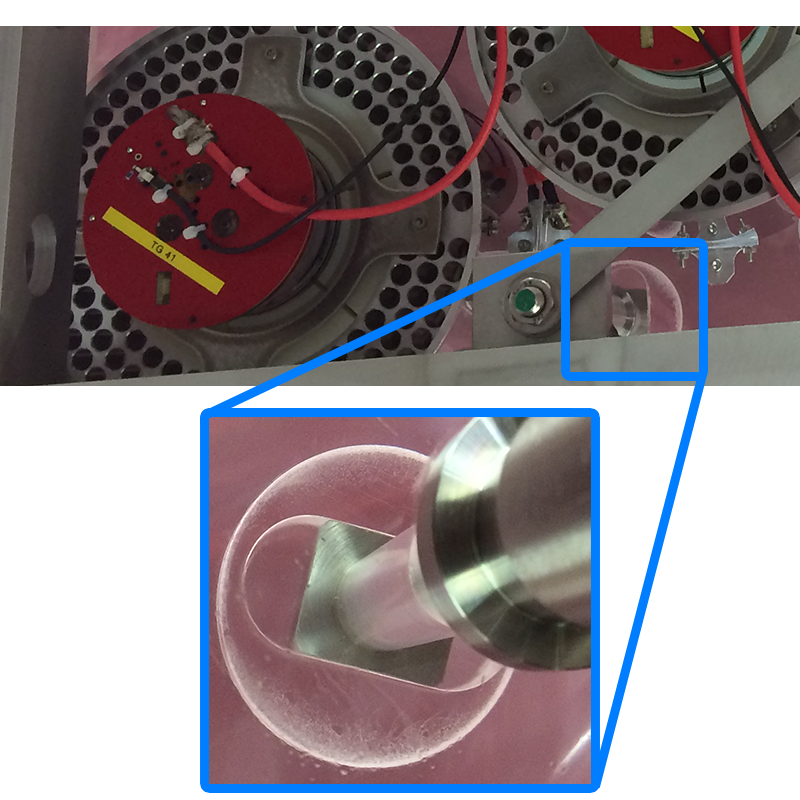
\includegraphics[width=0.75\linewidth]{images/buffer_repair.png} 
% \captionof{figure}[Photo du \textit{buffer} endommagé de la cellule 4]{Photo du \textit{buffer} endommagé de la cellule 4.} 
% \label{fig:buffer_repair.png} 
%\end{figure} 
% 
%\begin{figure}[h!] 
% \centering 
% \includegraphics[width=0.8\linewidth]{images/reflective_plates.png} 
% \captionof{figure}[]{.} 
% \label{fig:reflective_plates.png} 
%\end{figure} 
% 
%\clearpage 
%} 

%\begin{itemize} 
% \item Situation PN3, retrait de stéréo nécéssaire 
% \item Exposition des dégats / dégradations 
% \item Photos buffer 
% \item Réparations 
% \item Comportement Phase 2 
%\end{itemize} 

\subsection{Suivi et contrôle de la qualité des données} 
\label{sec:data_quality_control} 

Durant toute la période de prise de données, des mesures de stabilité et d'étalonnage ont été effectuées régulièrement: calibration de la réponse des PMs en photo-électrons, contrôle de l'homogénéité de la collection de lumière par les LEDs, calibration de la réponse en énergie du détecteur, suivi des paramètres de l'environnement de l'expérience.\\ 

À l'origine, les charges collectées par un photomultiplicateur $Q_{tot}$ sont exprimées dans des unités arbitraires (\og canaux ADC \fg{}), qui dépendent de paramètres différents à chaque PM : gain de la chambre d'amplification ou encore atténuation dans les câbles avant d'arriver aux Front-Ends. La correspondance canal ADC --- nombre de photo-électrons arrachés à la photocathode (PE) est établie en injectant une infime quantité de lumière dans le détecteur à l'aide de diodes. En pratique, l'acquisition est déclenchée par l'envoi du pulse de tension sur les diodes et un facteur d'amplification de 20 est utilisé pour ces triggers spécifiques afin de gagner en précision sur la réponse au photo-électron unique. L'intensité des diodes est ajustée de façon à ce que chaque événement enregistré n'ait déclenché en moyenne qu'une seule photo-avalanche dans chaque PM. La distribution obtenue en canaux ADC permet de déduire le facteur de conversion ADC vers PE (voire figure \ref{fig:pe_plot.pdf}). Cet étalonnage est effectué toutes les deux heures entre deux runs neutrino.\\ 

Après chaque calibration PE, une série de mesures est menée en injectant une plus grande quantité de lumière à différentes hauteurs dans le liquide: ce sont les runs LED. En plus de mesurer la stabilité de la réponse en PE, ces études permettent de contrôler l'évolution de la transparence du liquide ainsi que l'amplitude des fuites de lumière.\\ 

Le contrôle de la réponse en énergie du détecteur est effectué avec des sources radioactives gamma. Celles-ci sont déployées directement dans la Target par des tubes de calibration verticaux présents dans les cellules 1, 4 et 6 pour la Phase-I et 1, 2, 4, 5, 6 pour la Phase-II : c'est la calibration interne. Les sources peuvent aussi être déployées à l'extérieur pour étudier les effets de bords sur la collection de lumière. Pour ce faire, un \og pantographe \fg{} permet de faire circuler les sources radioactives autour du détecteur à différentes hauteurs. Un tube de calibration est aussi placé en dessous de la cuve dans le but de sonder la collection de lumière pour des dépôts d'énergie au fond des cellules. Les systèmes de calibration du détecteur sont représentés sur la figure \ref{fig:Calib_Systems.png}.\\

La calibration est étudiée tout particulièrement avec un échantillon de $\ce{^{54}Mn}$, car c'est une source intense mono gamma, c'est-à-dire un seul gamma émis à la fois, dont le parcours moyen d'environ 15 cm est comparable aux dimensions d'une cellule. Une session de calibration interne est menée chaque semaine pour suivre la réponse en énergie de chaque cellule avec cette source. L'échelle en énergie est plus généralement contrainte avec d'autres sources gamma: $\ce{^{68}Ge}$, $\ce{^{124}Sb}$, $\ce{^{137}Cs}$, $\ce{^{65}Zn}$, $\ce{^{60}Co}$, $\ce{^{42}K}$, $\ce{^{24}Na}$ ou encore l'$\ce{AmBe}$. Ces sources permettent de couvrir des énergies allant de \SI{511}{keV} à plus de \SI{4}{MeV}. Des campagnes de mesure complètes, impliquant des calibrations internes et externes, sont menées sur une base trimestrielle. En parallèle, des études dédiées à la détection des neutrons sont conduites à l'aide de la source d'$\ce{AmBe}$. Ces dernières ont pour objectif de contrôler la forme des cascades gamma du gadolinium ainsi que de mesurer précisément l'efficacité de détection des neutrons.\\ 

Quotidiennement, des suivis généraux sur l'état et l'environnement du détecteur sont pris en charge par une personne de la collaboration à tour de rôle (appelé \og \textit{shifter} \fg{}). La température extérieure, le niveau des liquides, le flux de neutrons, ou encore la pression atmosphérique sont mesurés grâce à des capteurs indépendants et les valeurs sont enregistrées sur une base de données MySQL. De même, des mesures fournies par l'ILL telles que la puissance réacteur, ou le niveau d'eau de la piscine au-dessus de \textsc{Stereo} sont stockées. Un site web a été développé pour contrôler l'évolution de tous les paramètres\footnote{\url{https://lpsc.in2p3.fr/stereo/WebSite/}}, et chaque jour le \textit{shifter} désigné atteste la qualité des données acquises et reporte les éventuelles anomalies dans un carnet de notes électronique ELog\footnote{\url{https://lpsc.in2p3.fr/elog/Stereo/}}. Pendant la première phase de prise données les \textit{shifter} étaient conviés à effectuer une visite sur site chaque jour afin de vérifier le bon fonctionnement de \textsc{Stereo}: hautes tensions des photomultiplicateurs, état des cartes d'acquisition, enregistrement sur disque dur, visualisation des spectres en charge, transfert des données sur les fermes de stockage, contrôle des alarmes automatiques, pression d'azote injectée, ou bien absence de fuites de liquides. Depuis le milieu de la Phase-II, ces tâches sont effectuées en remote par webcams et VNC. Le personnel local (LPSC ou ILL) se charge du contrôle sur site.\\ 

\afterpage{ 

\begin{figure}[h!] 
\centering 
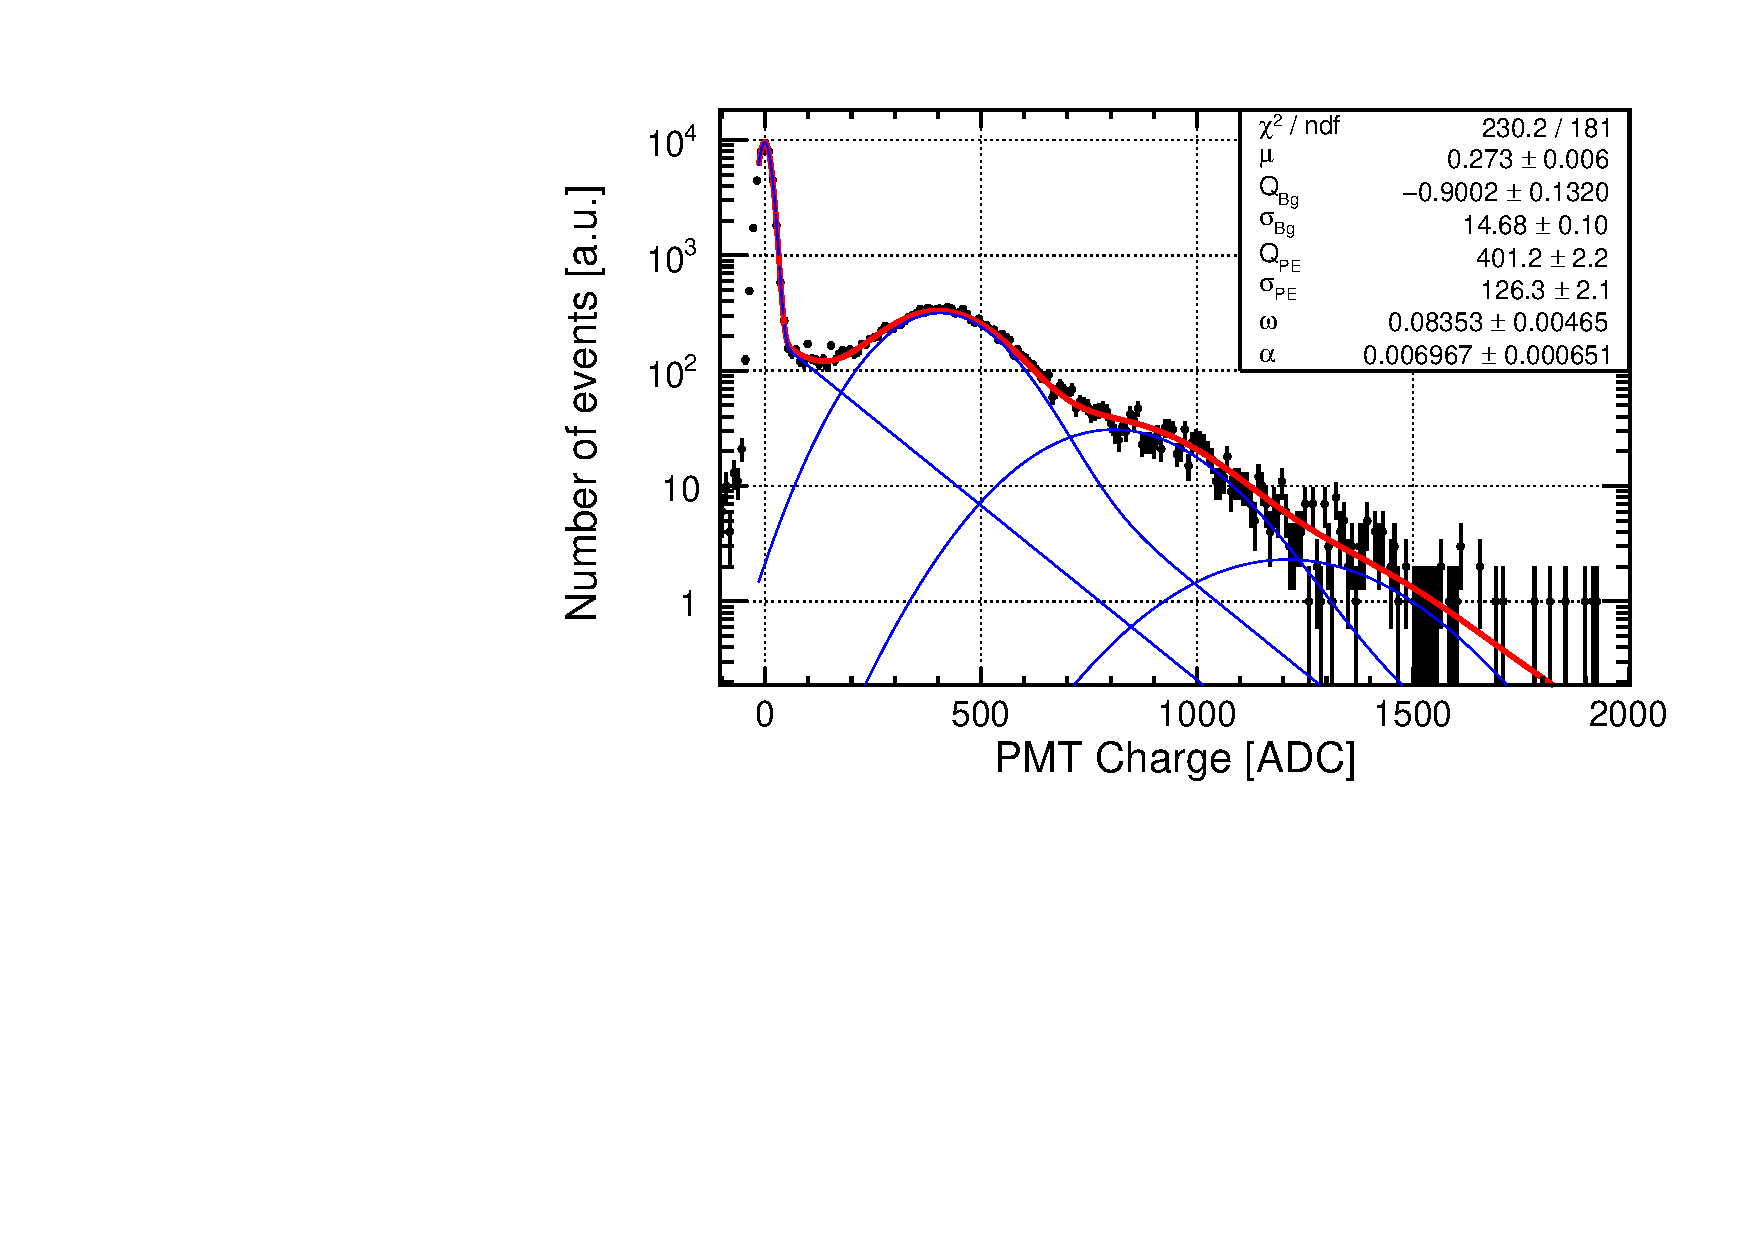
\includegraphics[width=1\linewidth]{images/pe_plot.pdf} 
\caption[Étalonnage de la réponse d'un photomultiplicateur]{Étalonnage de la réponse d'un photomultiplicateur. Le paramètre $Q_{\textrm{PE}}$ est ajusté sur les données et donne le numéro de canal ADC correspondant à un photo-électron arraché à la photocathode. La première gaussienne correspond au piédestal avec le bruit électronique, et les deux dernières sont présentes pour prendre en compte les contributions minoritaires à 2 ou 3 photo-électrons. (source \cite{Allemandou:2018vwb})} 
\label{fig:pe_plot.pdf} 
\end{figure} 

\begin{figure}[h!] 
\centering 
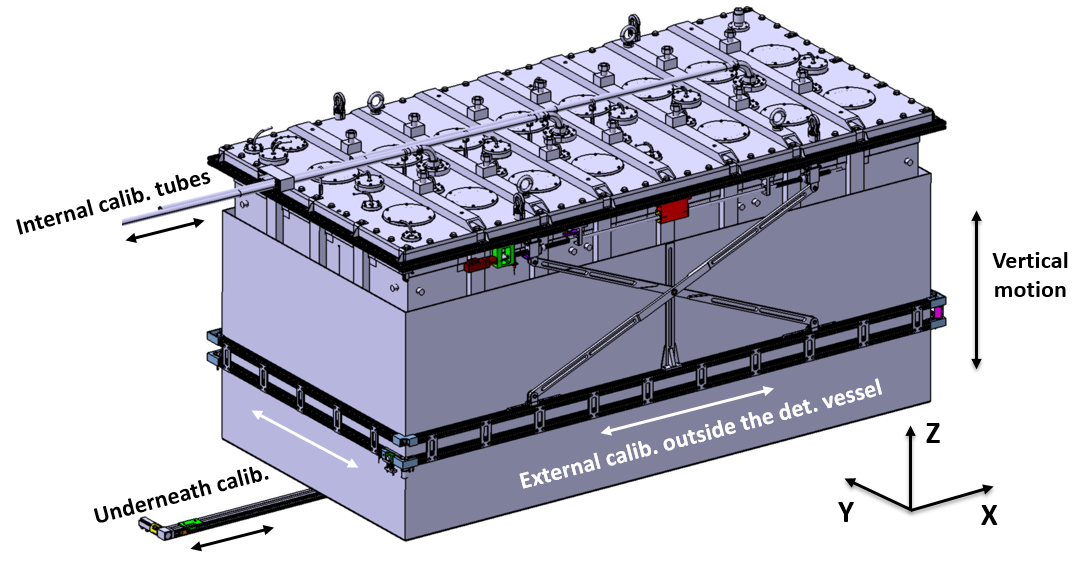
\includegraphics[width=1\linewidth]{images/Calib_Systems.png} 
\caption[Systèmes de calibration de la réponse en énergie du détecteur \textsc{Stereo}]{Systèmes de calibration de la réponse en énergie du détecteur \textsc{Stereo}. (source \cite{Allemandou:2018vwb})} 
\label{fig:Calib_Systems.png} 
\end{figure} 

\clearpage 

} 

\bigbreak 

%\begin{itemize} 
% \item Calibration PE 
% \item Calibration LED 
% \item Calibration sources Mn54 hédbo 
% \item Contrôle métrologie / HV / autre taches du shifter... 
%\end{itemize} 
